\documentclass{article}

\usepackage{arxiv}

\usepackage[utf8]{inputenc} % allow utf-8 input
\usepackage[T1]{fontenc}    % use 8-bit T1 fonts
\usepackage{lmodern}        % https://github.com/rstudio/rticles/issues/343
\usepackage{hyperref}       % hyperlinks
\usepackage{url}            % simple URL typesetting
\usepackage{booktabs}       % professional-quality tables
\usepackage{amsfonts}       % blackboard math symbols
\usepackage{nicefrac}       % compact symbols for 1/2, etc.
\usepackage{microtype}      % microtypography
\usepackage{graphicx}

\title{Novel Generation of Purely Synthetic Educational Dataset Effective For Research Applications}

\author{
    Austin Nicolas
    \thanks{The author's previous work that generated the dataset analyzed in this work can be found here \url{https://github.com/austineamonn/SummerResearch2024}}
   \\
    Department of Biology \\
    Grinnell College \\
  Grinnell, IA 50122 \\
  \texttt{\href{mailto:nicolasa@grinnell.edu}{\nolinkurl{nicolasa@grinnell.edu}}} \\
  }


% tightlist command for lists without linebreak
\providecommand{\tightlist}{%
  \setlength{\itemsep}{0pt}\setlength{\parskip}{0pt}}

% From pandoc table feature
\usepackage{longtable,booktabs,array}
\usepackage{calc} % for calculating minipage widths
% Correct order of tables after \paragraph or \subparagraph
\usepackage{etoolbox}
\makeatletter
\patchcmd\longtable{\par}{\if@noskipsec\mbox{}\fi\par}{}{}
\makeatother
% Allow footnotes in longtable head/foot
\IfFileExists{footnotehyper.sty}{\usepackage{footnotehyper}}{\usepackage{footnote}}
\makesavenoteenv{longtable}

% Pandoc citation processing
%From Pandoc 3.1.8
% definitions for citeproc citations
\NewDocumentCommand\citeproctext{}{}
\NewDocumentCommand\citeproc{mm}{%
  \begingroup\def\citeproctext{#2}\cite{#1}\endgroup}
\makeatletter
 % allow citations to break across lines
 \let\@cite@ofmt\@firstofone
 % avoid brackets around text for \cite:
 \def\@biblabel#1{}
 \def\@cite#1#2{{#1\if@tempswa , #2\fi}}
\makeatother
\newlength{\cslhangindent}
\setlength{\cslhangindent}{1.5em}
\newlength{\csllabelwidth}
\setlength{\csllabelwidth}{3em}
\newenvironment{CSLReferences}[2] % #1 hanging-indent, #2 entry-spacing
 {\begin{list}{}{%
  \setlength{\itemindent}{0pt}
  \setlength{\leftmargin}{0pt}
  \setlength{\parsep}{0pt}
  % turn on hanging indent if param 1 is 1
  \ifodd #1
   \setlength{\leftmargin}{\cslhangindent}
   \setlength{\itemindent}{-1\cslhangindent}
  \fi
  % set entry spacing
  \setlength{\itemsep}{#2\baselineskip}}}
 {\end{list}}
\usepackage{calc}
\newcommand{\CSLBlock}[1]{#1\hfill\break}
\newcommand{\CSLLeftMargin}[1]{\parbox[t]{\csllabelwidth}{#1}}
\newcommand{\CSLRightInline}[1]{\parbox[t]{\linewidth - \csllabelwidth}{#1}\break}
\newcommand{\CSLIndent}[1]{\hspace{\cslhangindent}#1}

\usepackage{tabularx}
\usepackage{amsmath}
\usepackage{multirow}
\begin{document}
\maketitle


\begin{abstract}
The research applications of currently available education datasets are limited by ethical concerns due to privacy loss revealing sensitive information about the students in the datasets. Current educational research uses machine learning to augment and analyze the currently available datasets. In parallel, in silico research is developing purely synthetic datasets generated based on empirical datasets. When carefully handled, these datasets can effectively limits privacy loss concerns. A purely synthetic dataset was developed for use in educational research by sampling from known distributions and creating novel mappings (Nicolas \& Sakib, 2024). However, no testing was done to compare the dataset to the original sampling distributions. This work examines the dataset to see if data generation aligned with sampling distributions and if weighted mappings effectively correlated features. We found that the generative function mostly sampled and mapped effectively to create significant correlations and distributions. Thus, the purely synthetic dataset mostly matches empirical data when such correlations and distributions were encoded in the generation function and the dataset, with some changes, can be used for educational research cases without privacy loss.
\end{abstract}

\keywords{
    synthetic data generation
   \and
    educational research
  }

\section{Introduction}\label{introduction}

In the past 20 years, educational research has begun using machine learning and artificial intelligence for a wide variety of purposes. The most common uses are for computer assisted instruction, virtual reality, tutoring systems, and augmented reality, which combined make up over 70\% of recent educational research in artificial intelligence and machine learning (Guan et al., 2020). However some educators warn that data driven approaches cannot replace educator experience and intuition, raising concerns about overreliance on artificial intelligence and machine learning outputs for determining educational policy and practices (Mandinach \& Schildkamp, 2021). These works almost always use empirical data which can leak private information about students despite data privatization practices.

Synthetic datasets have been uplifted as an alternative to empirical data for data augmentation purposes and to limit privacy loss. However, synthetic datasets are not automatically private, with privacy leakage risks of the data used to generate the synthetic dataset (Jordon et al., 2022). Thus, purely synthetic datasets are not based on specific empirical datasets have arisen as a solution to privacy loss concerns. Recent in silico work has used purely synthetic data in a wide variety of ways, including improving machine learning algorithm training speed (Gonsior et al., 2021), restoring resolution to degraded low resolution images (Wang et al., 2021), and annotating medical images (Liu et al., 2024).

One recent study used machine learning to predict future courses that university students would be interested in based on previous classes taken (Shao et al., 2021). More recently, a similar study was conducted that used a purely synthetic dataset based on known distributions and novel feature mappings rather than real world data that could be traced back to real students (Nicolas \& Sakib, 2024). Nicolas and Sakib developed a novel technique to generate the purely synthetic educational dataset for educational research purposes. Nicolas and Sakib focused on the privacy loss implications under several data privatization methods rather than the accuracy of the purely synthetic dataset. This work takes the dataset and examines if the generating function worked as the authors had intended.

We hypothesize that the data generation function from Nicolas \& Sakib (2024) functioned as intended. To support this hypothesis, we test whether observed feature distribution fits the sampled empirical distributions and whether features are correlated with eachother. Our first prediction is that dataset feature distributions will match the empirical sampling distribution. Next, we predict that the explicitly mapped features will be correlated. We also predict that the converse of the second prediction will be true. In other words, all features that were not explicitly mapped together will not be correlated.

\begin{table}[htbp]
  \centering
  \begin{tabular}{|l|l|}
    \hline
    Hypothesis & The data generation function worked as intended. \\ \hline
    Prediction 1 & Dataset feature distributions will match the empirical sampling distribution. \\ \hline
    Prediction 2 & Explicitly mapped features will be correlated. \\ \hline
    Converse of Prediction 2 & Non explicitly mapped features will not be correlated. \\ \hline
  \end{tabular}
  \caption{Hypothesis and Predictions.}
  \label{tab:hypothesis_predictions}
\end{table}

\section{Methods}\label{methods}

First, initial data preparation was done on the two datasets and then functions were developed to streamline the analysis process. Finally, Demographics, Majors, and Learning Styles were analyzed to see if the observed distribution matched the expected distribution and if features were correlated with one another. Here is a quick outline of this section:

\begin{enumerate}
\def\labelenumi{\arabic{enumi}.}
\tightlist
\item
  Datasets (\ref{sec:datasets})
\item
  Data Preparation (\ref{sec:data_preparation})
\item
  Demographics (\ref{sec:demographics})
\item
  Major (\ref{sec:major})
\item
  Learning Style (\ref{sec:learning_style})
\item
  Complex Correlations (\ref{sec:complex_correlations})
\end{enumerate}

Before we explain the methodology of the paper we quickly overview the datasets involved in the work.

\subsection{Datasets}\label{datasets}

\label{sec:datasets}

There were two datasets used in this analysis, both of which were generated in a paper by Nicolas \& Sakib (2024). The \emph{Purely Synthetic Education Dataset} was created by a novel generating function while the \emph{Majors Dataset} was created by webscrapping data from {``College {Majors Explorer}''} (n.d.).

\subsubsection{Purely Synthetic Education Dataset}\label{purely-synthetic-education-dataset}

The \emph{Purely Synthetic Education Dataset} was generated by sampling from known distributions or randomly selecting when distributions were unknown. Additionally, novel mappings were built between different columns to reflect known connections (Nicolas \& Sakib, 2024). The flowchart (Figure ref\{fig:data\_generation\}) shows the process used for generating each observation in the dataset.



\begin{figure}

{\centering 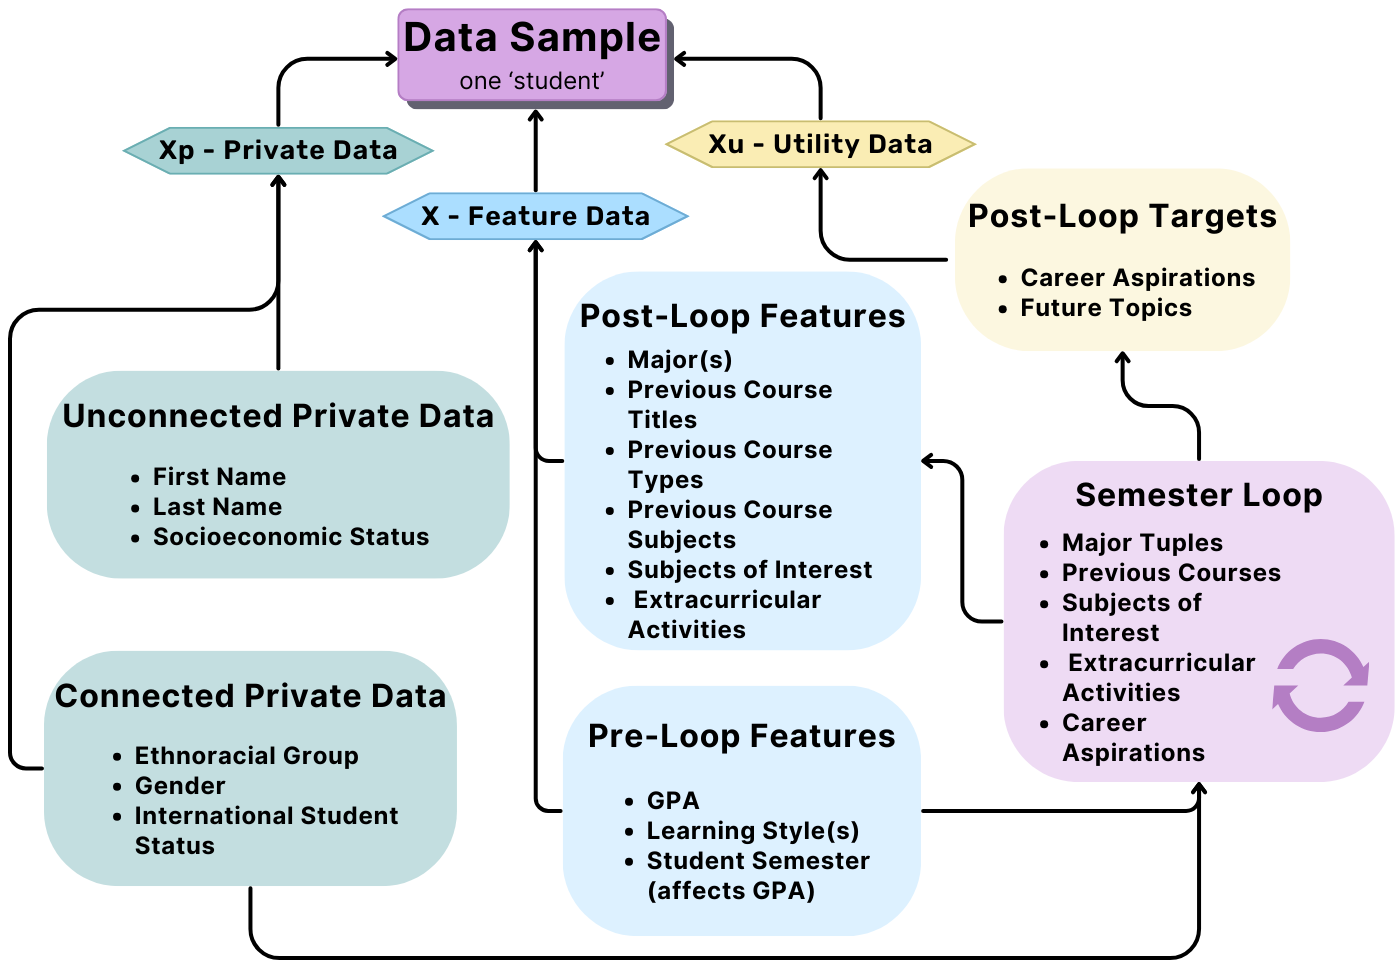
\includegraphics[width=0.9\linewidth]{data_generation_flowchart} 

}

\caption{This data generation flowchart was taken from (Nicolas \& Sakib, 2024).\label{fig:data_generation}}\label{fig:nicolas2024}
\end{figure}

Table \ref{tab:features_table} from Nicolas \& Sakib (2024) showcases the different features of the dataset. In this work, \textbf{Ethnoracial Group}, \textbf{Gender}, \textbf{International Student Status}, \textbf{Socioeconomic Status}, \textbf{GPA}, \textbf{Learning Style(s)}, \textbf{Student Semester}, \textbf{Major(s)}, \textbf{Previous Course Types}, and \textbf{Previous Course Subjects}, were analyzed.

\begin{table}[htbp]
    \centering
    \begin{tabular}{|l|l|l|l|}
        \hline
        \textbf{Features} & \textbf{Data Category} & \textbf{Data Type} & \textbf{Number of Options}\\ \hline
        First Name & $X_p$ & String & 32,952 \\ \hline
        Last Name & $X_p$ & String & 151,671 \\ \hline
        Ethnoracial Group & $X_p$ & String & 7 \\ \hline
        Gender & $X_p$ & String & 3 \\ \hline
        International Student Status & $X_p$ & String & 2 \\ \hline
        Socioeconomic Status & $X_p$ & String & 5 \\ \hline
        GPA & X & Double & 201 \\ \hline
        Learning Style(s) & X & List of Strings & 4 \\ \hline
        Student Semester & X & Integer & 15 \\ \hline
        Major(s) & X & List of Strings & 173 \\ \hline
        Previous Course Titles & X & List of Strings & 3,476 \\ \hline
        Previous Course Types & X & List of Strings & 21 \\ \hline
        Previous Course Subjects & X & List of Strings & 236 \\ \hline
        Subjects of Interest & X & List of Strings & 141 \\ \hline
        Extracurricular Activities & X & List of Strings & 304 \\ \hline
        Career Aspirations & $X_u$ & List of Strings & 149 \\ \hline
        Future Topics & $X_u$ & List of Strings & 226 \\ \hline
    \end{tabular}
    \caption{Information about Data Features.}
    \label{tab:features_table}
\end{table}

Table \ref{tab:first_row_transposed} shows the first row of the dataset. The row was transposed and the long string list columns were concatenated to prevent the row from running of the page.

\begin{table}[htbp]
  \centering
  \begin{tabular}{|l|l|}
    \hline
    \textbf{Column Name} & \textbf{First Entry} \\ \hline
    First name & Raycen \\ \hline
    Last Name & Tallini \\ \hline
    Ethnoracial Group & European American or white \\ \hline
    Gender & Female \\ \hline
    International Student Status & International \\ \hline
    Socioeconomic Status & Middle Income \\ \hline
    Learning Style & {[}'Read/Write'{]} \\ \hline
    GPA & 3.86 \\ \hline
    Student Semester & 10 \\ \hline
    Major & {[}'Teacher Education: Multiple Levels'{]} \\ \hline
    \multirow{2}{*}{Previous Courses} & {[}'Intensive Elementary Spanish', 'General Chemistry Lab II', \\
    & \ldots, 'Advanced Study Abroad'{]} \\ \hline
    \multirow{2}{*}{Course Types} & {[}{[}'Laboratory-Discussion', 'Lecture', 'Practice'{]}, \\
    & {[}'Lecture-Discussion', 'Online'{]},\ldots, {[}'Discussion/Recitation', 'Lecture'{]}{]} \\ \hline
    Course Subjects & {[}'ACES', 'EPOL', 'GWS',\ldots, 'ART'{]} \\ \hline
    Subjects of Interest & {[}'History', 'Philosophy',\ldots, 'Engineering'{]} \\ \hline
    \multirow{2}{*}{Extracurricular Activities} & {[}'Education Society', 'Engineering Society', \\
    & \ldots, 'Electrical Engineering Club'{]} \\ \hline
    \multirow{2}{*}{Career Aspirations} & {[}'Postsecondary Teacher', 'Other Teacher and Instructor', \\
    & \ldots, 'Material Engineer'{]} \\ \hline
  \multirow{2}{*}{Future Topics} & {[}'Leadership Studies', 'Sociology', \\
  & \ldots, 'Human Development and Family Studies'{]} \\ \hline
  \end{tabular}
  \caption{The first row of the dataset, transposed. Long list features concatenated.}
  \label{tab:first_row_transposed}
\end{table}

\subsubsection{Majors Dataset}\label{majors-dataset}

The Majors Dataset was stored as a JSON file so it was imported using the JSONlite package (Ooms et al., 2024). Table \ref{tab:majors_dataset} shows the features of the \emph{Majors Dataset} from Nicolas \& Sakib (2024), who based it on a data webscrapped from {``College {Majors Explorer}''} (n.d.).

\begin{table}[htbp]
  \centering
  \begin{tabular}{|l|l|l|}
    \hline
    Data Column & Data Type & Data From \\
    \hline
    Major & String & Majors List \\
    \hline
    National Percent Female & float & Represents a percentage so between 0 and 1 \\
    \hline
    Popularity Ranking & Integer & Between 1 and 173 \\
    \hline
    Division & Factor & One of 6 Divisions\\
    \hline
    Top 5 Careers & List of Strings & Careers List\\
    \hline
  \end{tabular}
  \caption{Majors Dataset}
  \label{tab:majors_dataset}
\end{table}

The \emph{Majors Dataset} contains the following major divisions: Business, Education, Health, Liberal Arts, Social Sciences, and STEM.

\subsection{Data Preparation}\label{data-preparation}

\label{sec:data_preparation}

The preprocessing pipelines for the features analyzed in this work are summarized in Table \ref{tab:data_prep_table}.

\begin{table}[htbp]
    \centering
    \begin{tabular}{|l|l|l|l|}
        \hline
        \textbf{Features} & \textbf{Rename Column} & \textbf{Convert to a Factor} & \textbf{Split Lists and Recombine}\\ \hline
        Ethnoracial Group & YES & YES & NO \\ \hline
        Gender & YES & YES & NO \\ \hline
        International Student Status & YES & YES & NO \\ \hline
        Socioeconomic Status & YES & YES & NO \\ \hline
        GPA & YES & NO & NO \\ \hline
        Learning Style(s) & YES & NO & YES \\ \hline
        Student Semester & YES & NO & NO \\ \hline
        Major(s) & YES & NO & YES \\ \hline
        Previous Course Types & YES & NO & YES \\ \hline
        Previous Course Subjects & YES & NO & YES \\ \hline
    \end{tabular}
    \caption{Data Preparation Pipeline.}
    \label{tab:data_prep_table}
\end{table}

Renaming columns and converting to factors was done through Tidyverse (Wickham, 2023). Since the lists of strings in the \emph{Purely Synthetic Education Dataset} were stored as strings, they had to be stripped and split into multiple columns. This was done for \textbf{Learning Styles(s)}, \textbf{Major(s)}, \textbf{Previous Course Types}, and \textbf{Previous Course Subjects} but the same process could be applied to the other list of string features. Then each split column was put into its own copy of the \emph{Purely Synthetic Education Dataset} and they were recombined rowwise.

\subsubsection{Dictionary}\label{dictionary}

The Dict package (Asai, 2020) was used to create a dictionary with feature names as the keys and the column name for the feature as the values. The key and value for \textbf{Ethnoracial Group} are shown below:

\begin{quote}
Key: ``Ethnoracial Group'', Value: ``ethnoracial\_group''
\end{quote}

\subsection{Demographics}\label{demographics}

\label{sec:demographics}

The demographic section looks at the following 6 features:

\begin{enumerate}
\def\labelenumi{\arabic{enumi}.}
\tightlist
\item
  Ethnoracial Group
\item
  Gender
\item
  International Student Status
\item
  Socioeconomic Status
\item
  GPA
\item
  Student Semester
\end{enumerate}

The string demographics (\textbf{Ethnoracial Group}, \textbf{Gender}, \textbf{International Student Status}, and \textbf{Socioeconomic Status}) were sampled based on empirical data distributions. The numerical demographics (\textbf{GPA} and \textbf{Student Semester}) were sampled from a uniform distribution. All the demographics were sampled independently of one another (Nicolas \& Sakib, 2024).

\subsubsection{Statistical Testing}\label{statistical-testing}

The Chi Squared Goodness of Fit Test was run on \textbf{Ethnoracial Group}, \textbf{Gender}, \textbf{International Student Status}, and \textbf{Socioeconomic Status} comparing them with their known distributions. Known distributions were taken from Nicolas \& Sakib (2024).

The Chi Squared Test of Independence was run between \textbf{Ethnoracial Group}, \textbf{Gender}, \textbf{International Student Status}, and \textbf{Socioeconomic Status}.

\subsubsection{Graphing}\label{graphing}

For each combination of \textbf{Ethnoracial Group}, \textbf{Gender}, \textbf{International Student Status}, and \textbf{Socioeconomic Status} a bar chart comparing the proportion of one feature across the options for the other feature was created using ggplot2 (Wickham, 2023) and RColorBrewer (Neuwirth, 2022).

For \textbf{GPA} and \textbf{Student Semester} the number of students in a given semester or with a certain GPA were graphed with a horizontal line representing the expected uniform distribution of the features. This was done using ggplot2 (Wickham, 2023).

\subsection{Major}\label{major}

\label{sec:major}

The major function from Nicolas \& Sakib (2024) determined a student's major based on a weighting by gender and major popularity. For a major \(m\), let \(P_m\) be the popularity ranking of the major and let \(F_m\) be the percentage of female identifying students in the major. Since there are 173 majors we know that \(P_m\in[1,173]\cap\mathbb{N}\).

\[
W_m=1-\frac{P_m}{173}+\begin{cases} 
  1-\frac{F_m}{100} & \text{if student identifies as Male} \\
  \frac{F_m}{100} & \text{otherwise}
\end{cases}
\]

\subsubsection{Joining the Majors Dataset}\label{joining-the-majors-dataset}

A left join was used to combine the \emph{Majors Dataset} with the \emph{Purely Synthetic Education Dataset} where the \textbf{Major(s)} feature was split and recombined.

\subsubsection{Statistical Testing}\label{statistical-testing-1}

The Chi Squared Goodness of Fit Test was run on the popularity of each major vs the expected popularity ranking. The observed popularity was calculated by taking the number of students in each major (splitting double majors) and ranking them. The results were graphed in a bar graph using ggplot2 (Wickham, 2023) and viridis (Garnier et al., 2024).

The Chi Squared Test of Independence was run with \textbf{Majors(s)} against \textbf{Ethnoracial Group}, \textbf{Gender}, \textbf{International Student Status}, and \textbf{Socioeconomic Status}.

\subsubsection{Gender By Major}\label{gender-by-major}

Since \textbf{Gender} was the only feature that was explicitly called in the generating function for picking \textbf{Major(s)} then the Chi Squared Goodness of Fit test was run to compare the expected percent female of each major from the \emph{Majors Dataset} vs what was observed in the \emph{Purely Synthetic Education Dataset}. Then the dataset was filtered using Wickham (2023) to get the top ten majors with the highest percentage of male, female, and gender minority (female and nonbinary) students. Nonbinary students were never filtered alone since the sample size was too small. Then the results were graphed in a bar graph using ggplot2 (Wickham, 2023) and RColorBrewer (Neuwirth, 2022).

\subsection{Learning Style}\label{learning-style}

\label{sec:learning_style}

The learning style function from Nicolas \& Sakib (2024) determined a student's learning style(s) based on randomly sampling from a weighted distribution based on the empirical distribution of the learning styles. There is also a 10\% chance of a student getting a second learning style, though if it is a duplicate it is ignored.

\subsubsection{Statistical Testing}\label{statistical-testing-2}

The Chi Squared Goodness of Fit Test was run on the popularity of each learning style vs the expected distribution.

The Chi Squared Test of Independence was run with \textbf{Learning Style(s)} against \textbf{Ethnoracial Group}, \textbf{Gender}, \textbf{International Student Status}, and \textbf{Socioeconomic Status}.

\subsection{Complex Correlations}\label{complex-correlations}

\label{sec:complex_correlations}

The \texttt{pick\_classes} function from Nicolas \& Sakib (2024) determined a student's classes based on a list of classes with each class weighted as follows:

\begin{table}[htbp]
  \centering
  \begin{tabular}{|l|l|}
    \hline
    \textbf{Class matches Student's} & \textbf{Weighting} \\ \hline
    Learning Style(s) & 2 \\ \hline
    Major(s) & 5 \\ \hline
    Nothing & 1 \\ \hline
  \end{tabular}
  \caption{Class Weightings.}
  \label{tab:class_weightings}
\end{table}

Classes are based on a student's \textbf{Majors(s)} and \textbf{Learning Style(s)}. So, a student with a math major would be more likely to take a math course. From each class the course subject was taken (ex: MAT for a math class). Additionally, a student with a Read/Write learning style would be more likely to take courses that focus on reading and writing. From each class the course type was taken (ex: Lecture for a math class), with each course type being associated with one or more learning styles. Thus, we want to determine if there are correlations between these variables.

Take the joined dataset that was already split by \textbf{Major(s)} and split it by \textbf{Course Subjects}. Then recombine using the \texttt{rbind} function from base R. Then the Chi Squared Test Test of Independence is run to determine if \textbf{Major(s)} and \textbf{Course Subjects} are correlated.

Take the dataset that was already split by \textbf{Learning Style(s)} and split it by \textbf{Course Types}. Then recombine using the \texttt{rbind} function from base R. Then the Chi Squared Test Test of Independence is run to determine if \textbf{Learning Style(s)} and \textbf{Course Types} are correlated.

\section{Results}\label{results}

\begin{enumerate}
\def\labelenumi{\arabic{enumi}.}
\tightlist
\item
  Demographics (\ref{sec:demographics_res})
\item
  Major (\ref{sec:major_res})
\item
  Learning Style (\ref{sec:learning_style_res})
\item
  Complex Correlations (\ref{sec:complex_correlations_res})
\end{enumerate}

\subsection{Demographics}\label{demographics-1}

\label{sec:demographics_res}

First, we look at how well the demographic feature distribution fits the empirical data from which they were sampled. Then, we examine if the demographics are correlated together or if they are independent. Finally, we graph the numerical features (\textbf{GPA} and \textbf{Student Semester}) and compare them to the uniform distribution from which they were sampled.

\subsubsection{Distribution Fit}\label{distribution-fit}

Table \ref{tab:demographics_chi_gof} shows how well each of the feature distributions matched the empirical distribution. None of them were significant.

\begin{table}[htbp]
  \centering
  \begin{tabular}{|l|l|}
    \hline
    \textbf{Demographic} & \textbf{P-Value} \\ \hline
    Ethnoracial Group & 1 \\ \hline
    Gender & 1 \\ \hline
    International Student Status & 0.997 \\ \hline
    Socioeconomic Status & 1 \\ \hline
  \end{tabular}
  \caption{Chi Squared Goodness of Fit Test. *p<0.05}
  \label{tab:demographics_chi_gof}
\end{table}

\subsubsection{Demographic Correlations}\label{demographic-correlations}

Table \ref{tab:demographics_chi_indep} shows how well each of the features correlate with each other. None of them were significant. Though \textbf{Socioeconomic Status} and \textbf{International Student Status} were close to significant at p=0.08951.

\begin{table}[htbp]
  \centering
  \begin{tabular}{|l|l|l|l|}
    \hline
    \multicolumn{1}{|c|}{\multirow{2}{*}{}} &                 \multicolumn{1}{c|}{\multirow{2}{*}{Gender}} & \multicolumn{1}{c|}{International Student} & \multicolumn{1}{c|}{Socioeconomic} \\
    \multicolumn{1}{|c|}{} & \multicolumn{1}{c|}{} & \multicolumn{1}{c|}{Status} & \multicolumn{1}{c|}{Status} \\ \hline
    Ethnoracial Group & 0.8605 & 0.5301 & 0.5707 \\ \hline
    Gender &  & 0.1464 & 0.1799 \\ \hline
    International Student Status &  &  & 0.08951 \\ \hline
  \end{tabular}
  \caption{Chi Squared Test of Independence between Demographics. *p<0.05}
  \label{tab:demographics_chi_indep}
\end{table}

The correlation graph (Figure \ref{fig:demg0}) shows the correlation between ethnoracial group and gender and we see how similar the bars look.



\begin{figure}

{\centering 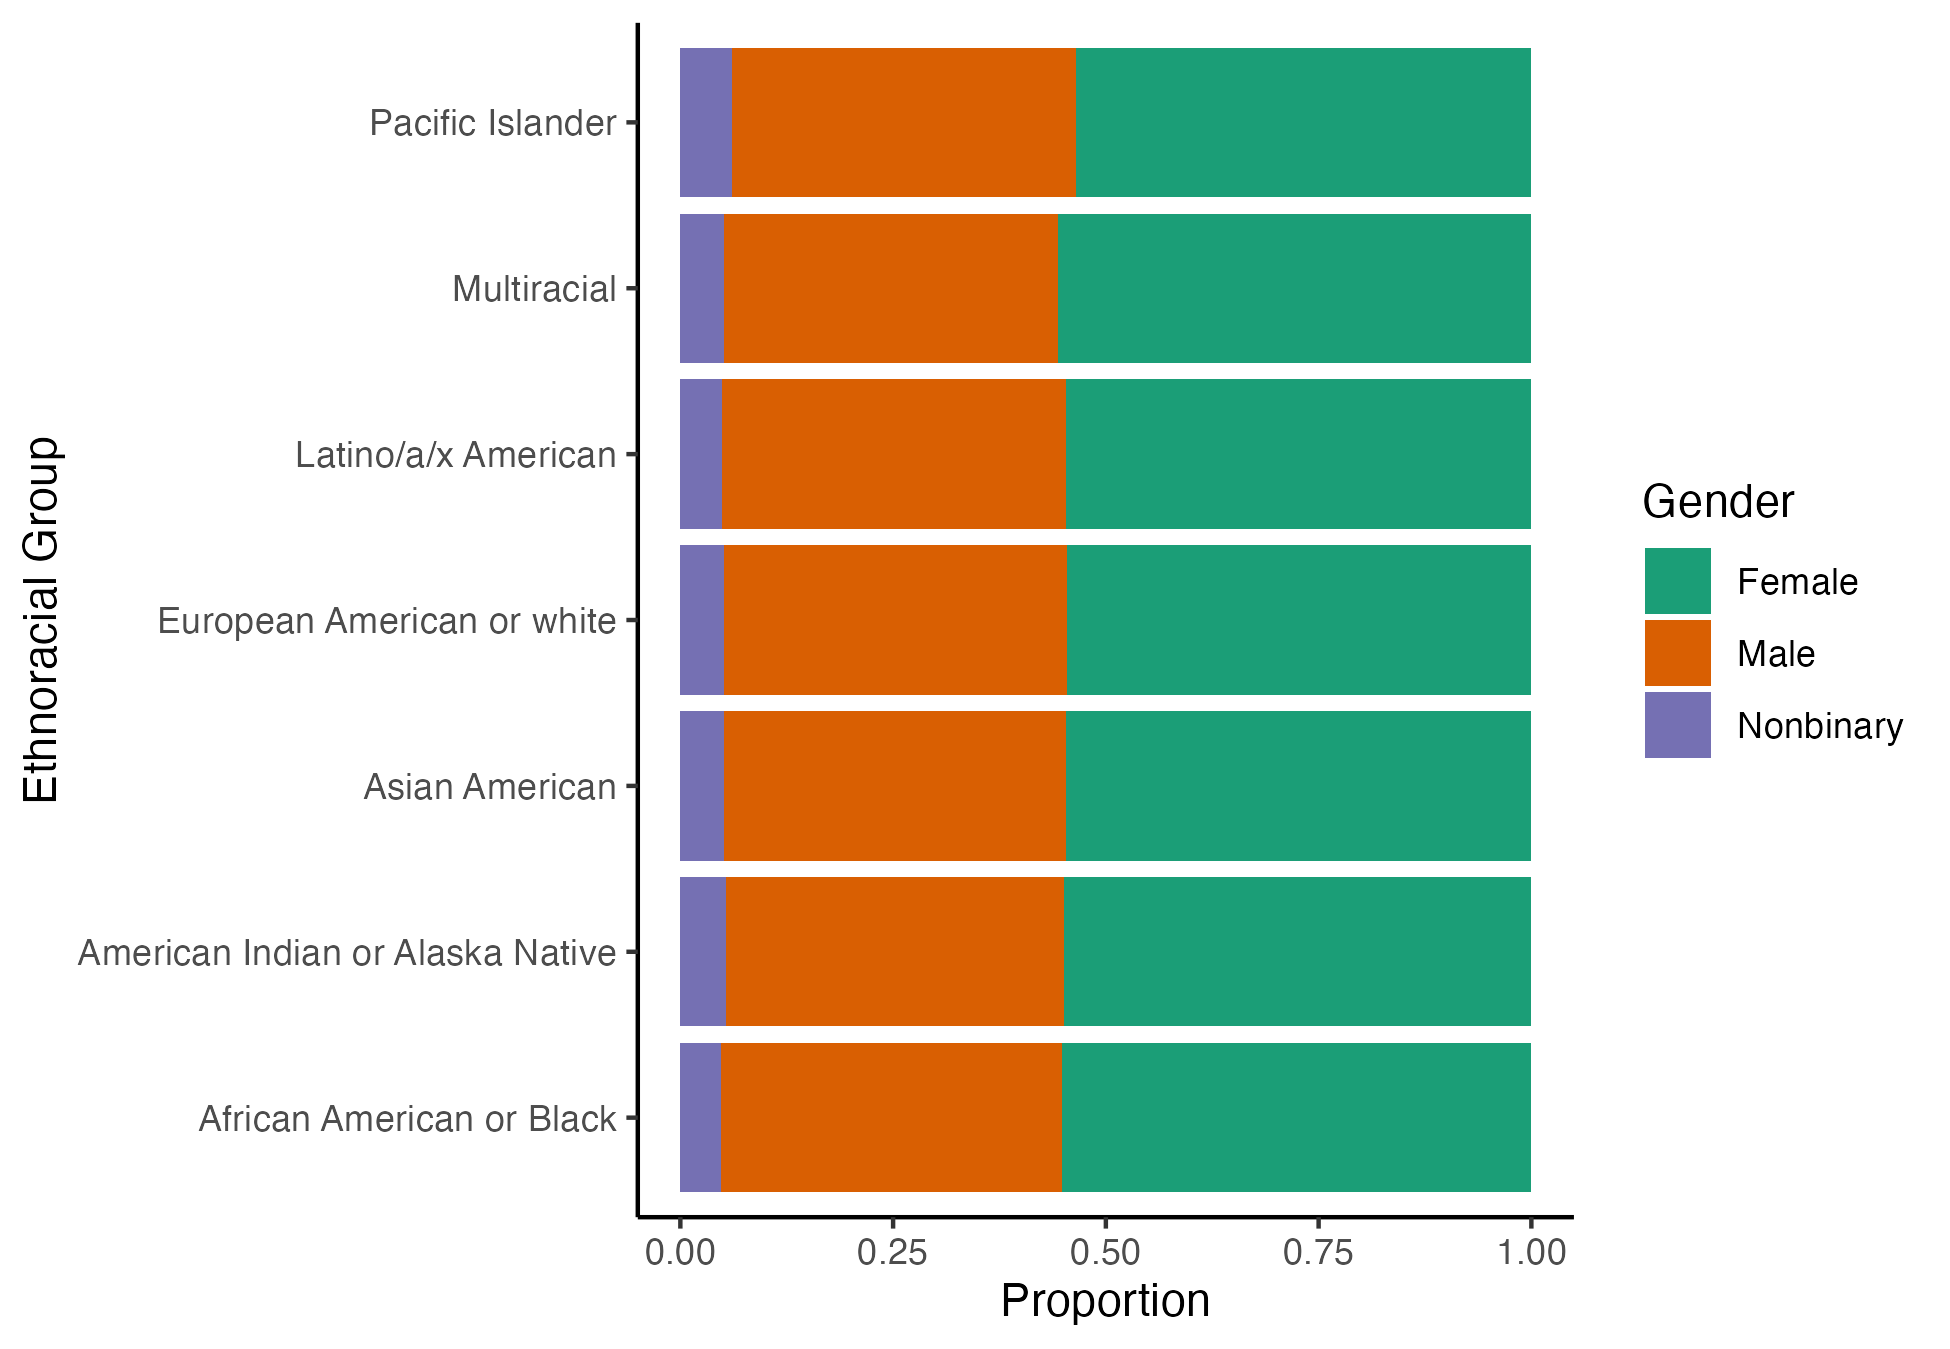
\includegraphics[width=0.9\linewidth]{ethnoracial_group_v_gender} 

}

\caption{Correlation graph between ethnoracial group and gender.}\label{fig:demg0}
\end{figure}

The correlation graph (Figure \ref{fig:demg1}) shows the correlation between ethnoracial group and international student status and we see how similar the bars look.



\begin{figure}

{\centering 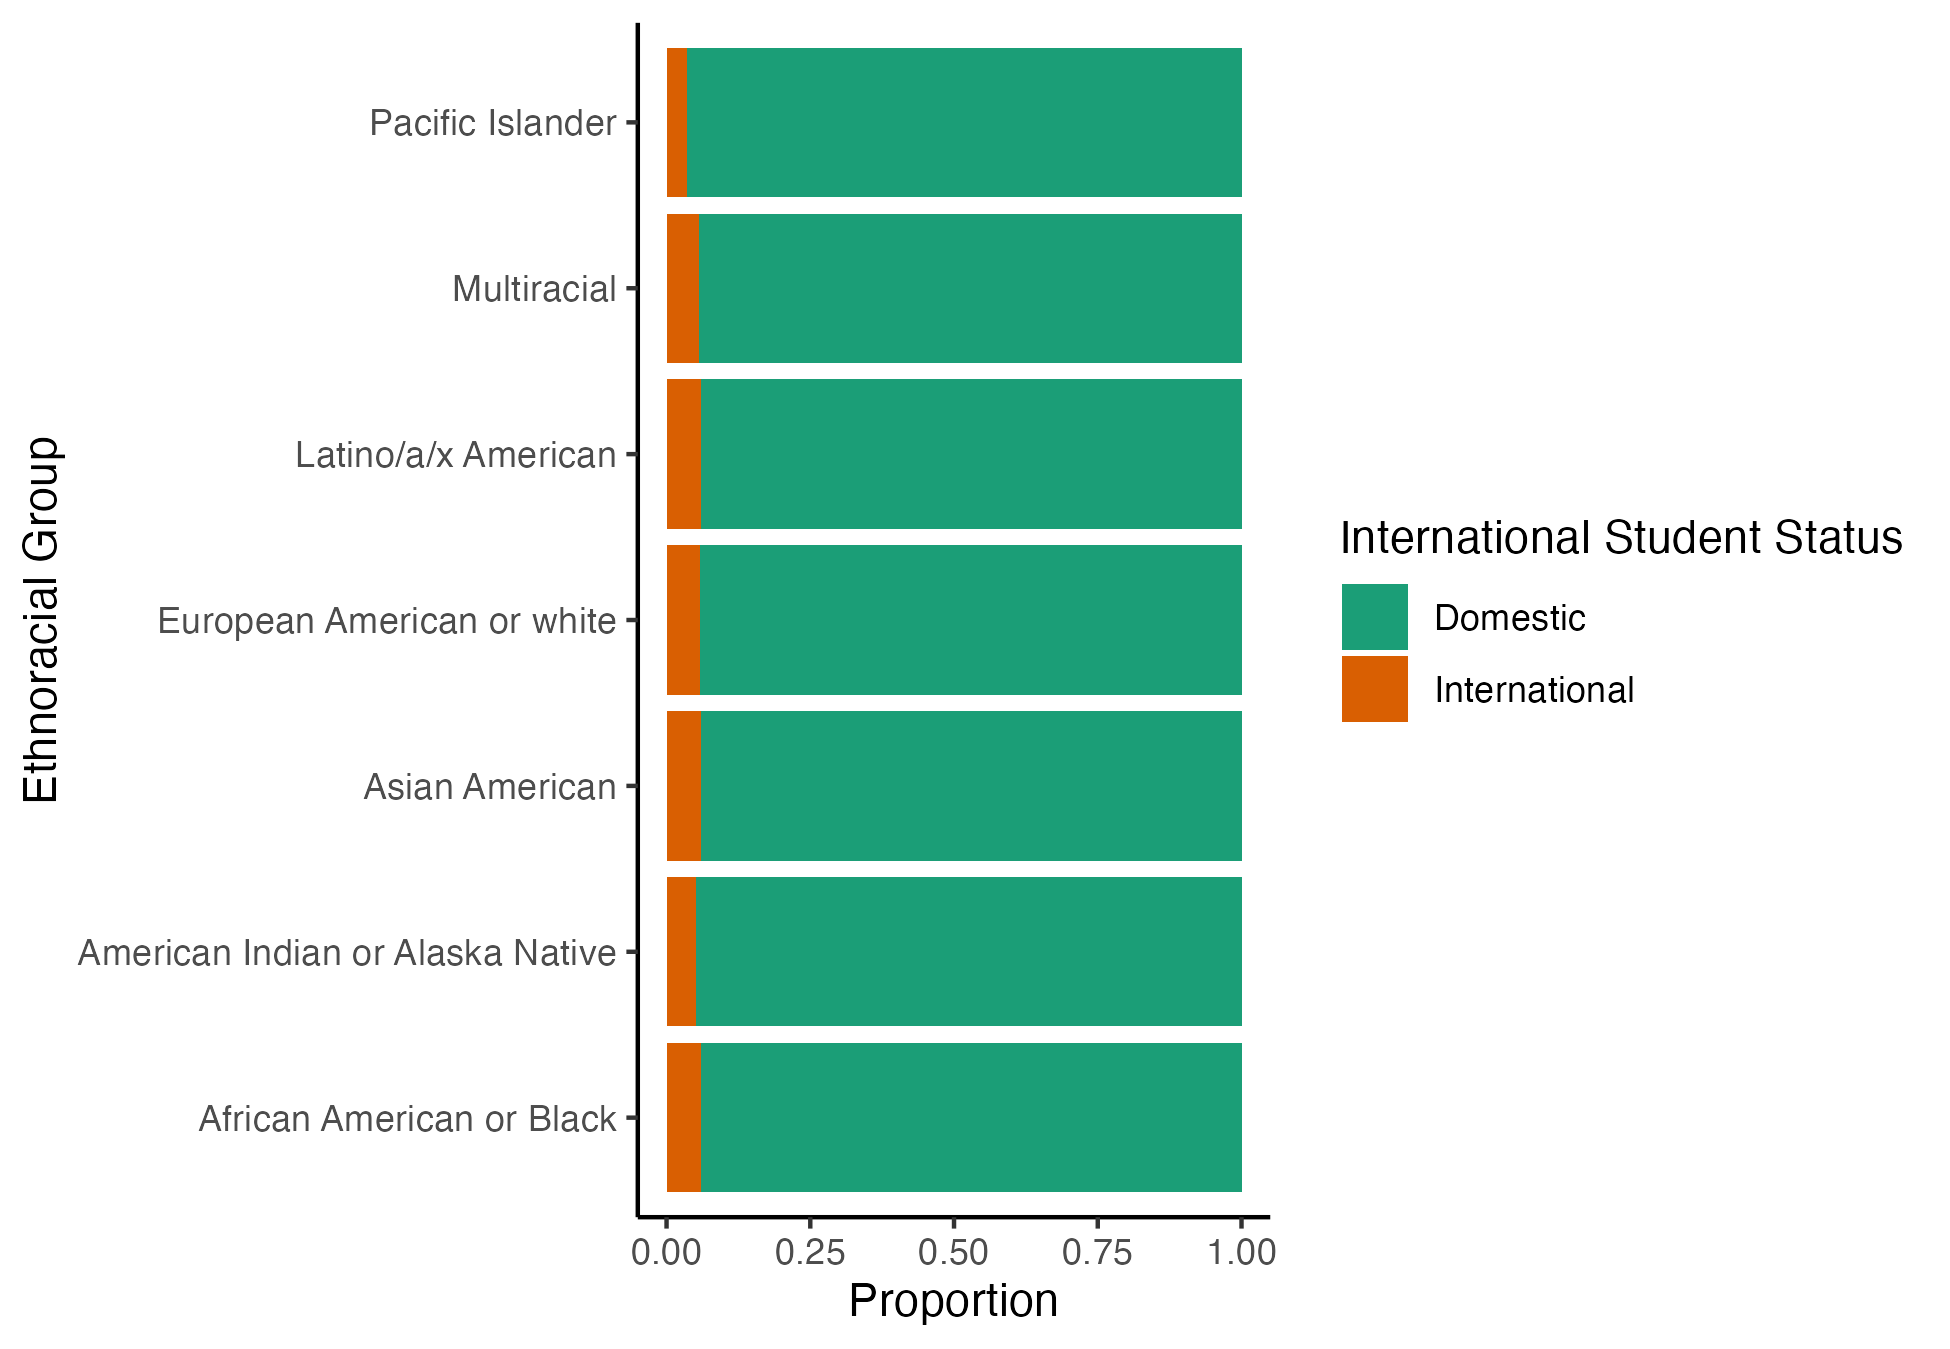
\includegraphics[width=0.9\linewidth]{ethnoracial_group_v_international_student_status} 

}

\caption{Correlation graph between ethnoracial group and international student status.}\label{fig:demg1}
\end{figure}

The correlation graph (Figure \ref{fig:demg0}) shows the correlation between ethnoracial group and socioeconomic status and we see how similar the bars look.



\begin{figure}

{\centering 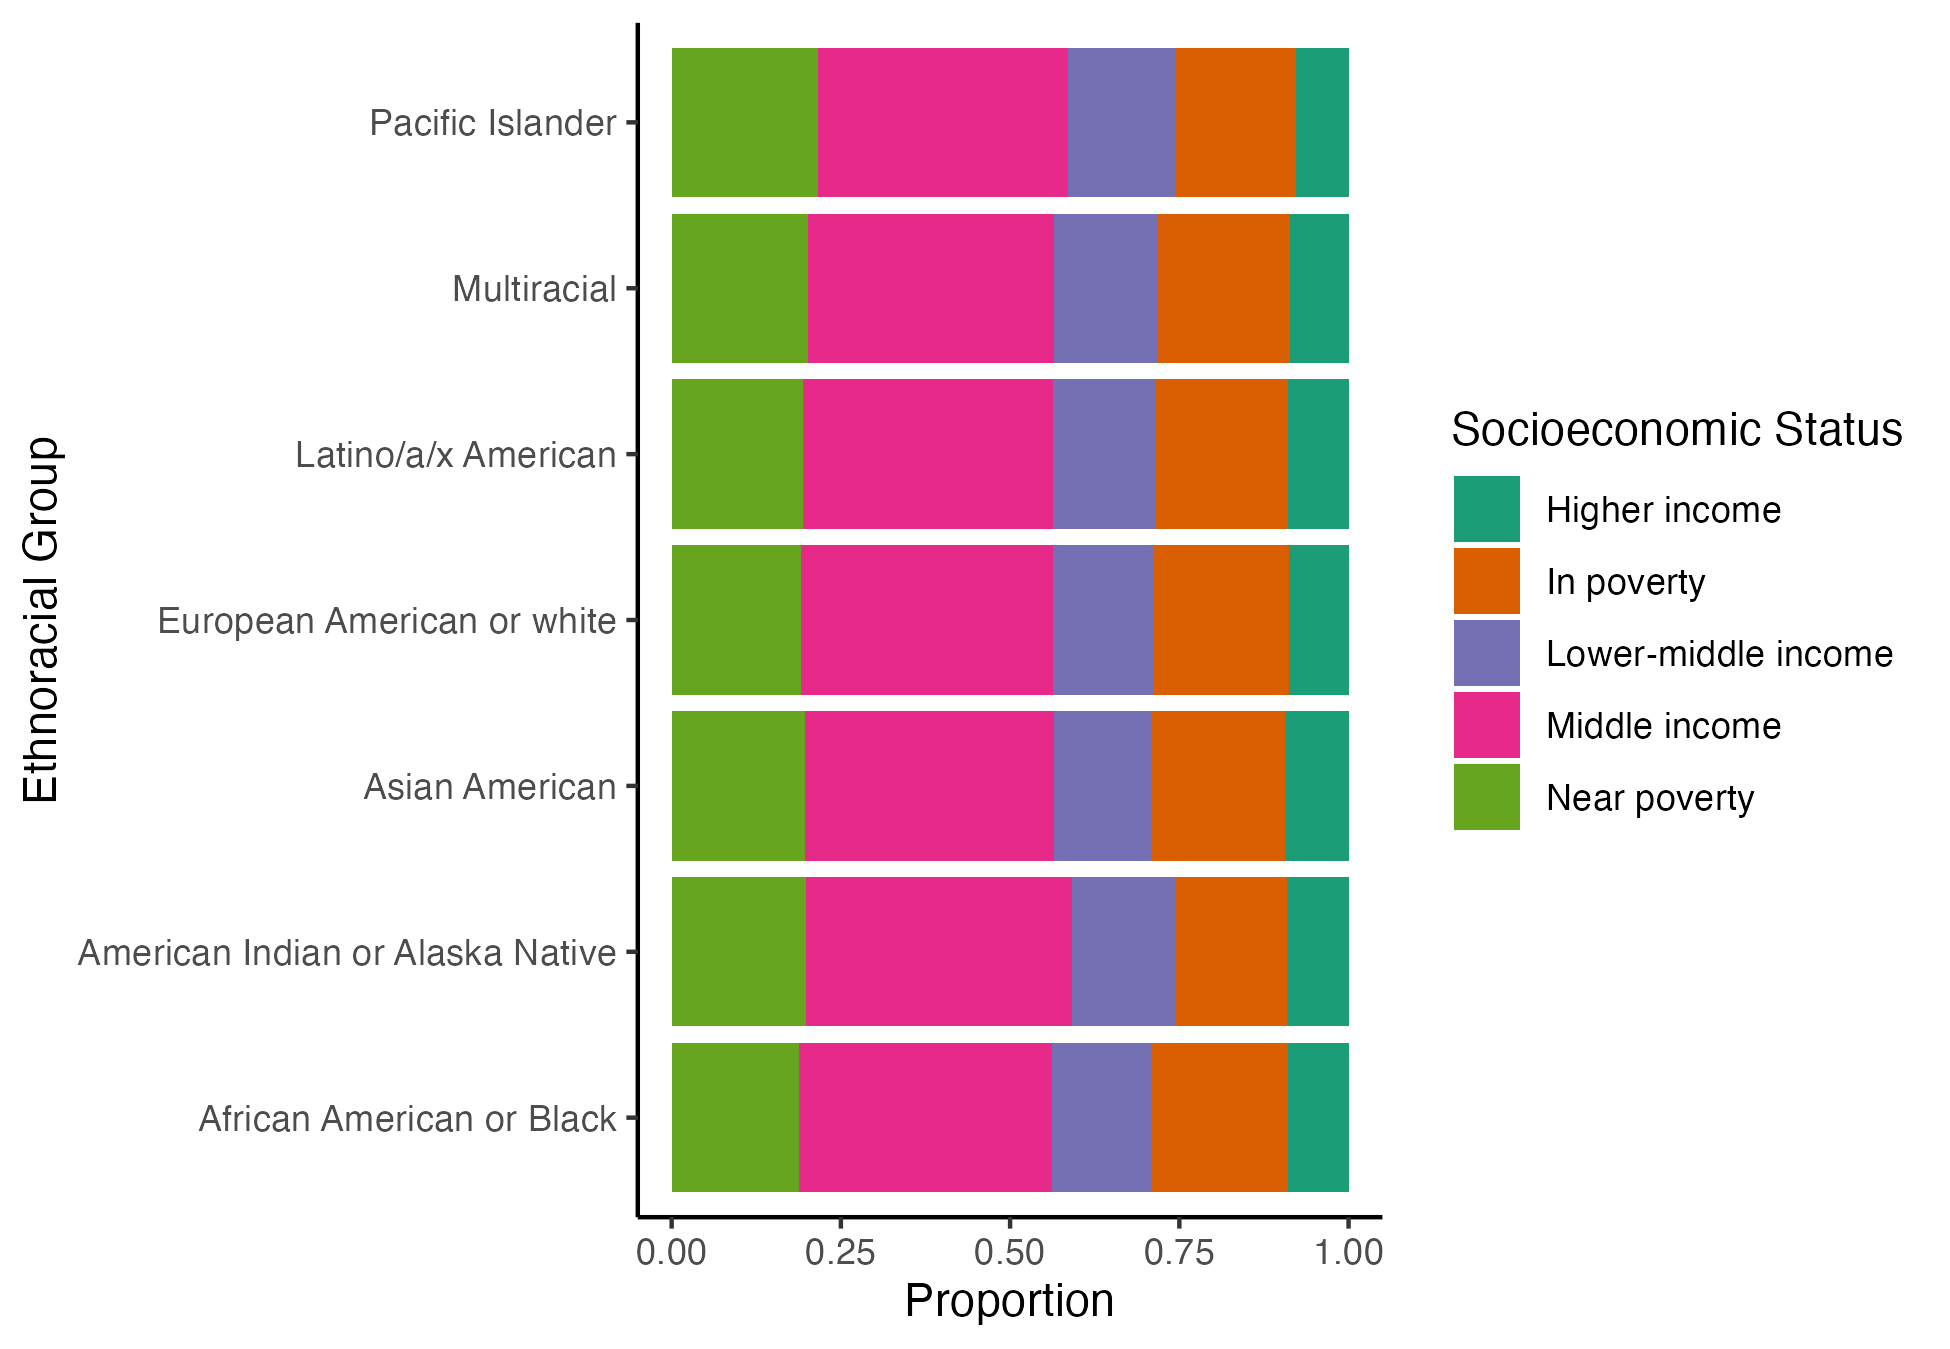
\includegraphics[width=0.9\linewidth]{ethnoracial_group_v_socioeconomic_status} 

}

\caption{Correlation graph between ethnoracial group and socioeconomic status.}\label{fig:demg2}
\end{figure}

The correlation graph (Figure \ref{fig:demg3}) shows the correlation between gender and international student status and we see how similar the bars look.



\begin{figure}

{\centering 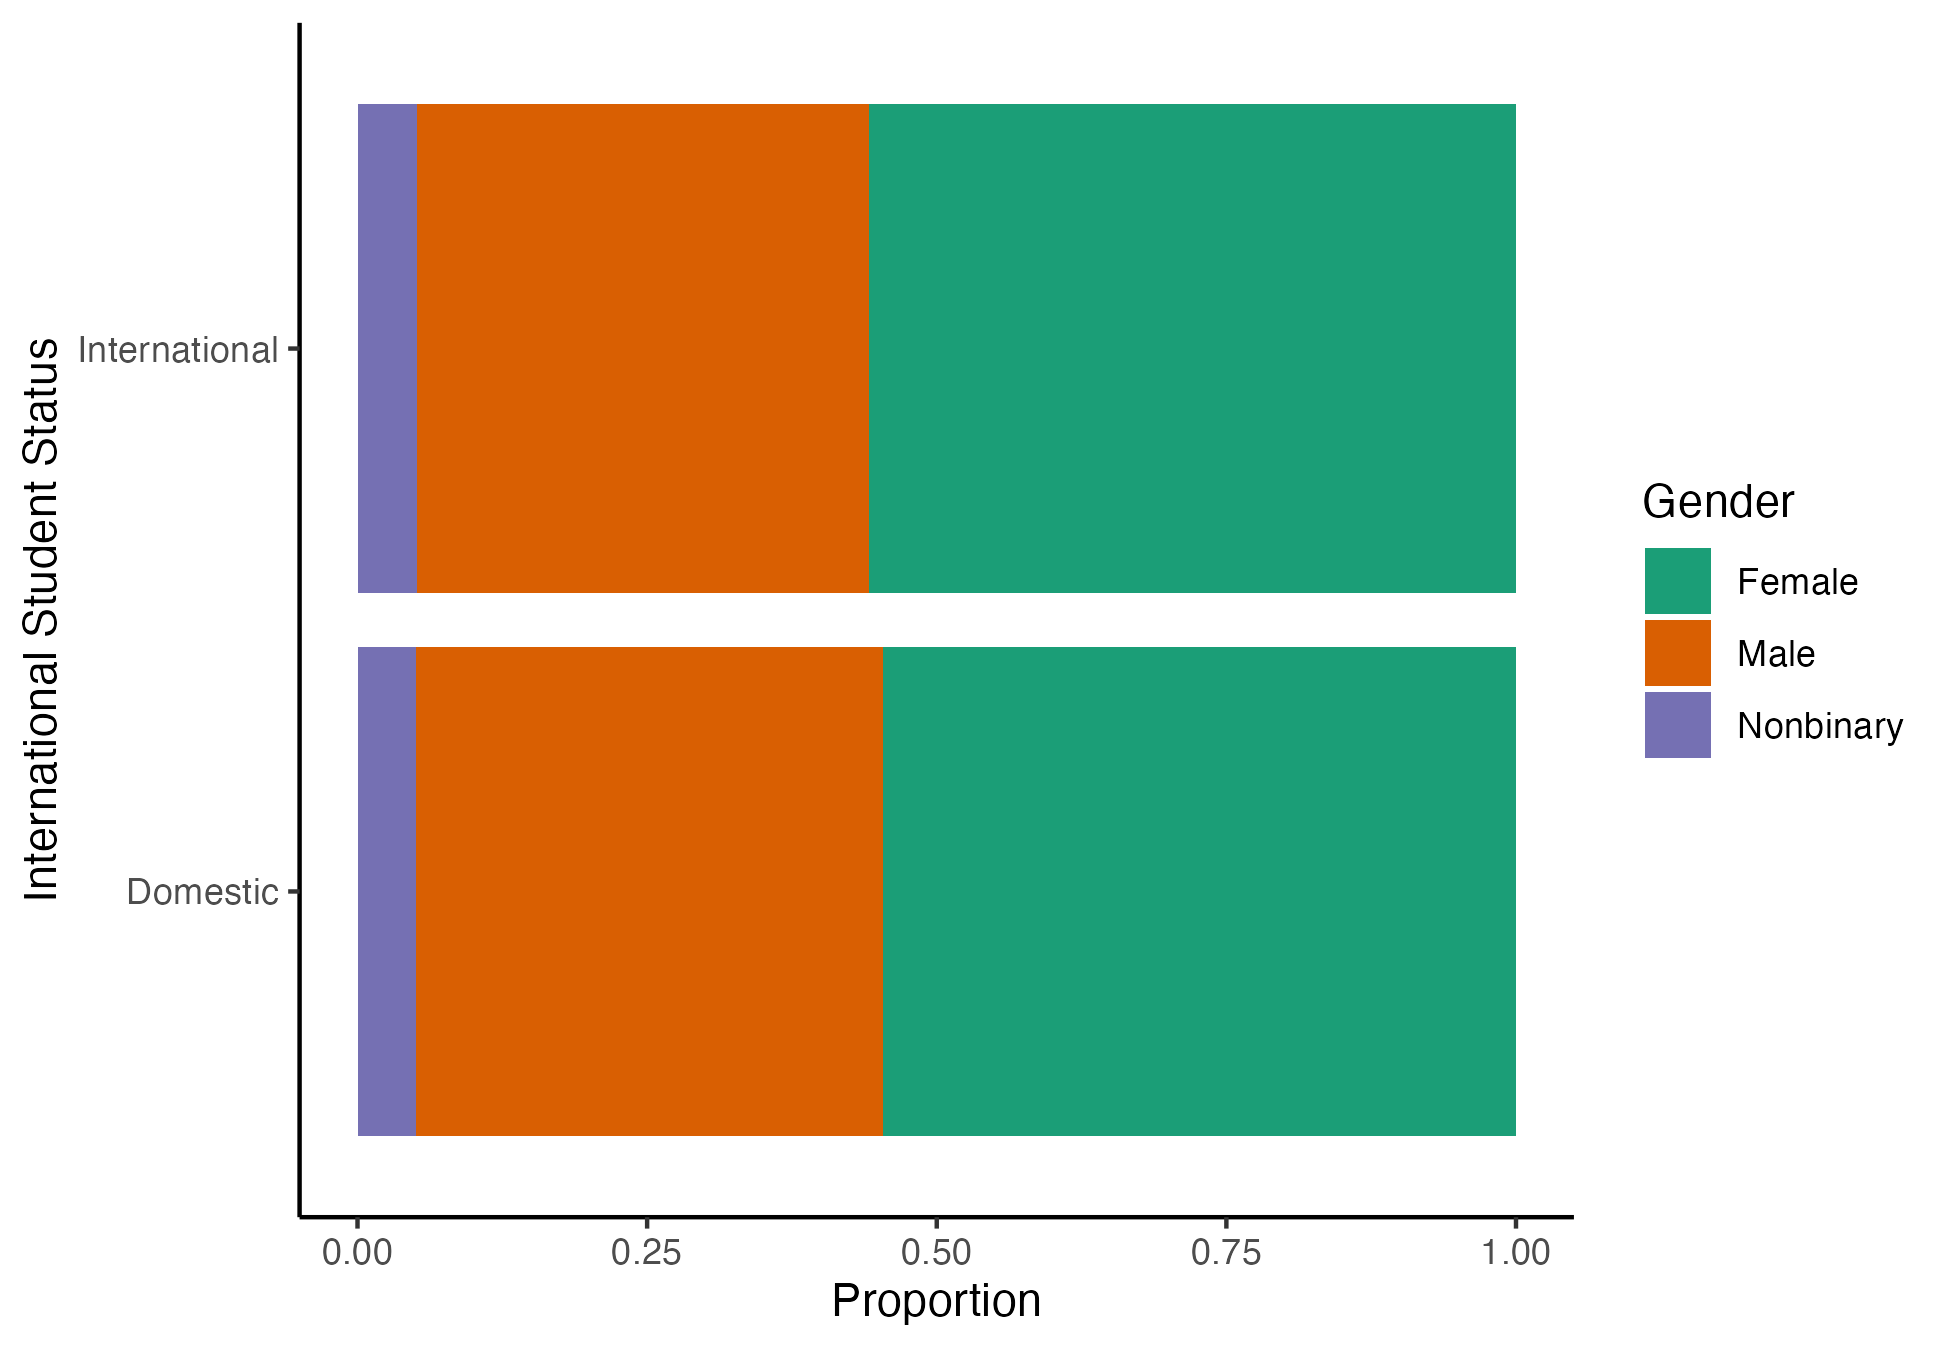
\includegraphics[width=0.9\linewidth]{gender_v_international_student_status} 

}

\caption{Correlation graph between gender and international student status.}\label{fig:demg3}
\end{figure}

The correlation graph (Figure \ref{fig:demg4}) shows the correlation between gender and socioeconomic status and we see how similar the bars look.



\begin{figure}

{\centering 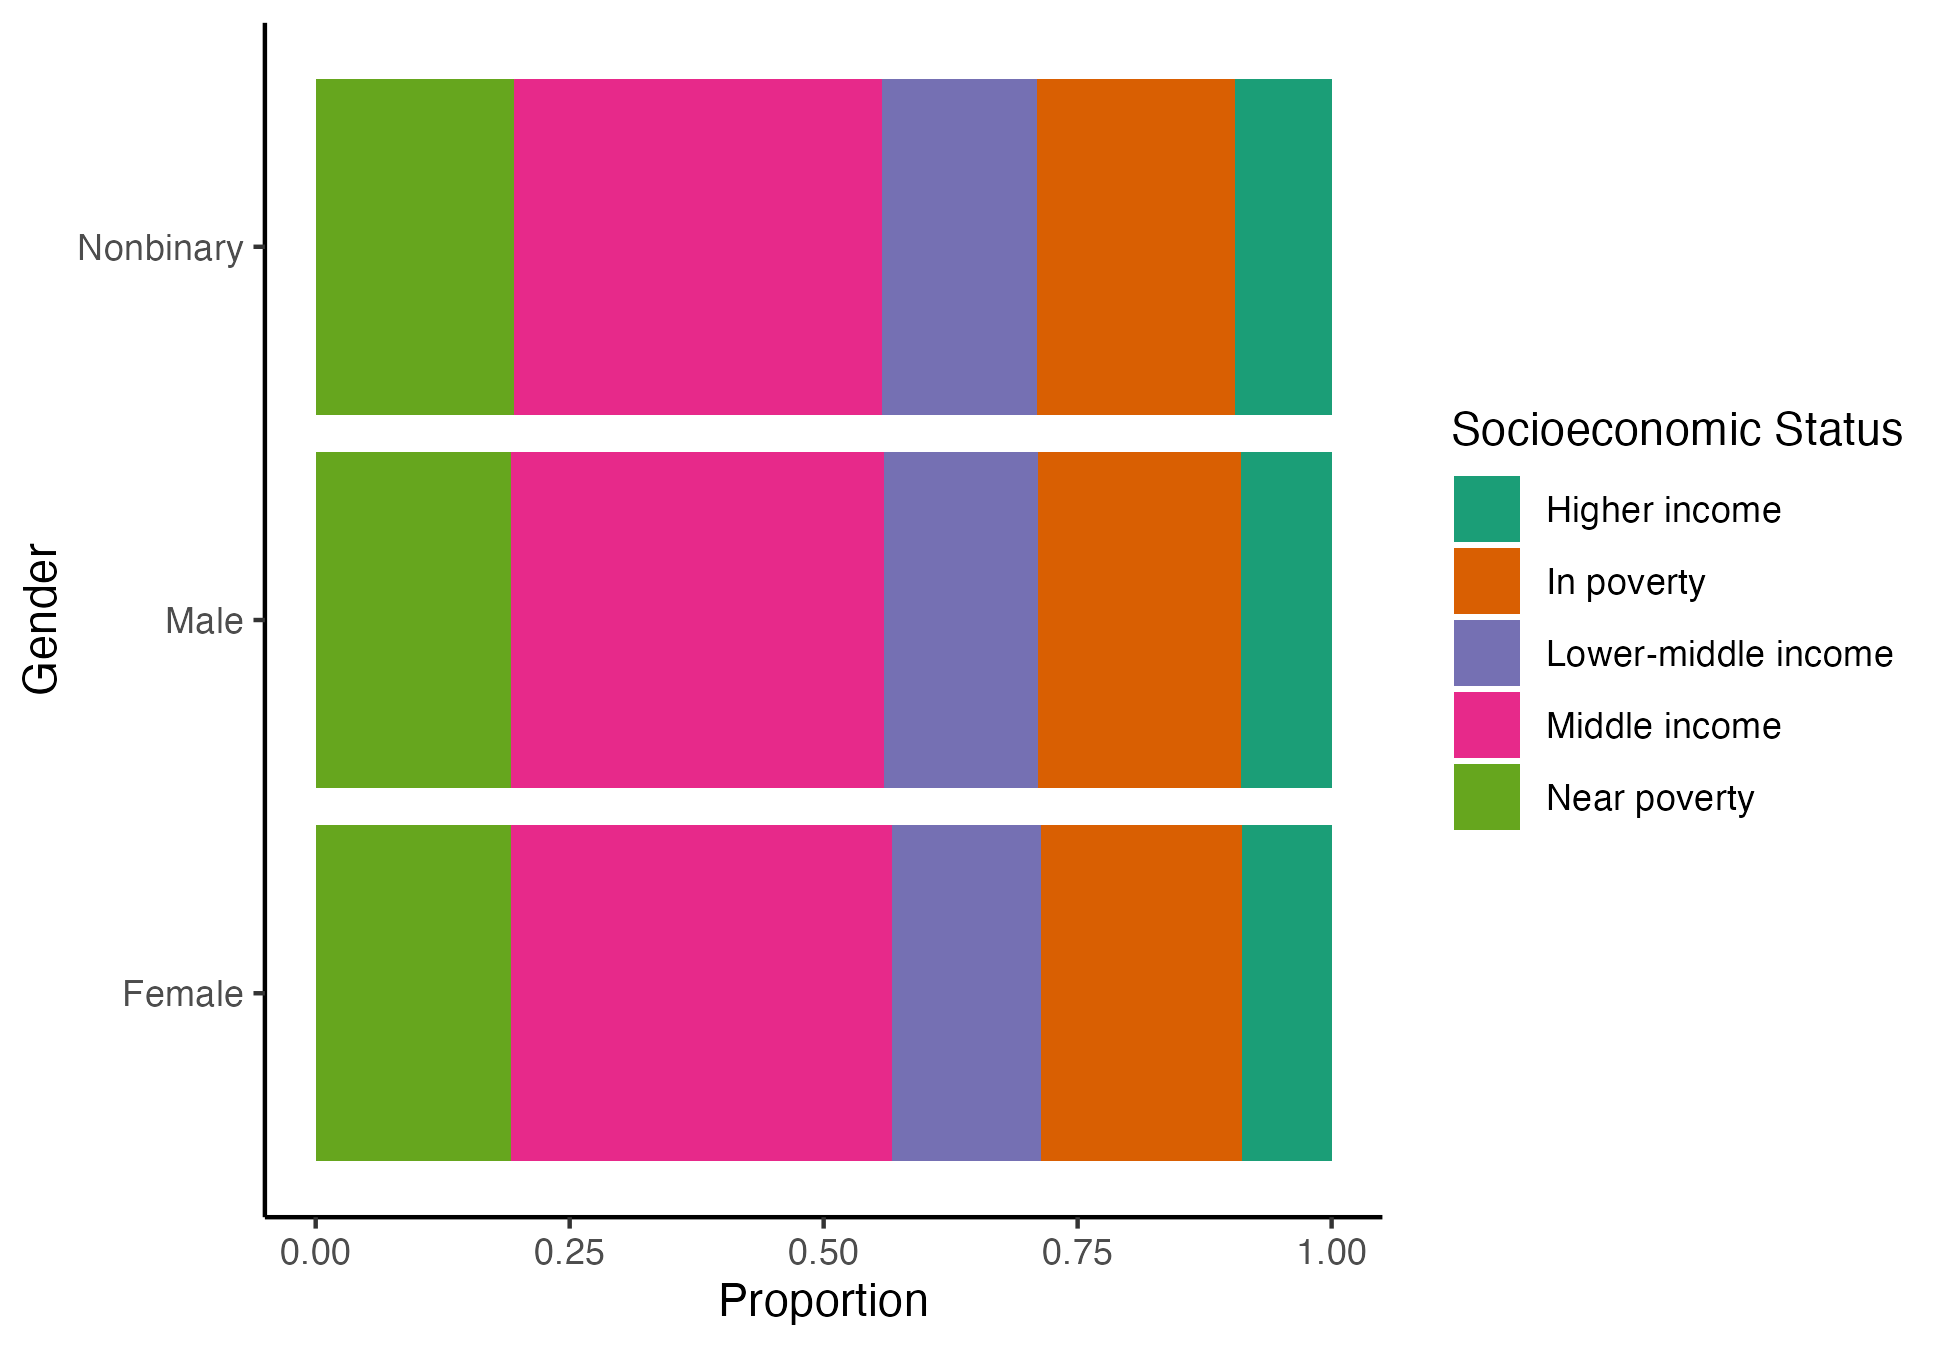
\includegraphics[width=0.9\linewidth]{gender_v_socioeconomic_status} 

}

\caption{Correlation graph between gender and socioeconomic status.}\label{fig:demg4}
\end{figure}

The correlation graph (Figure \ref{fig:demg5}) shows the correlation between international student status and socioeconomic status and we see how similar the bars look.



\begin{figure}

{\centering 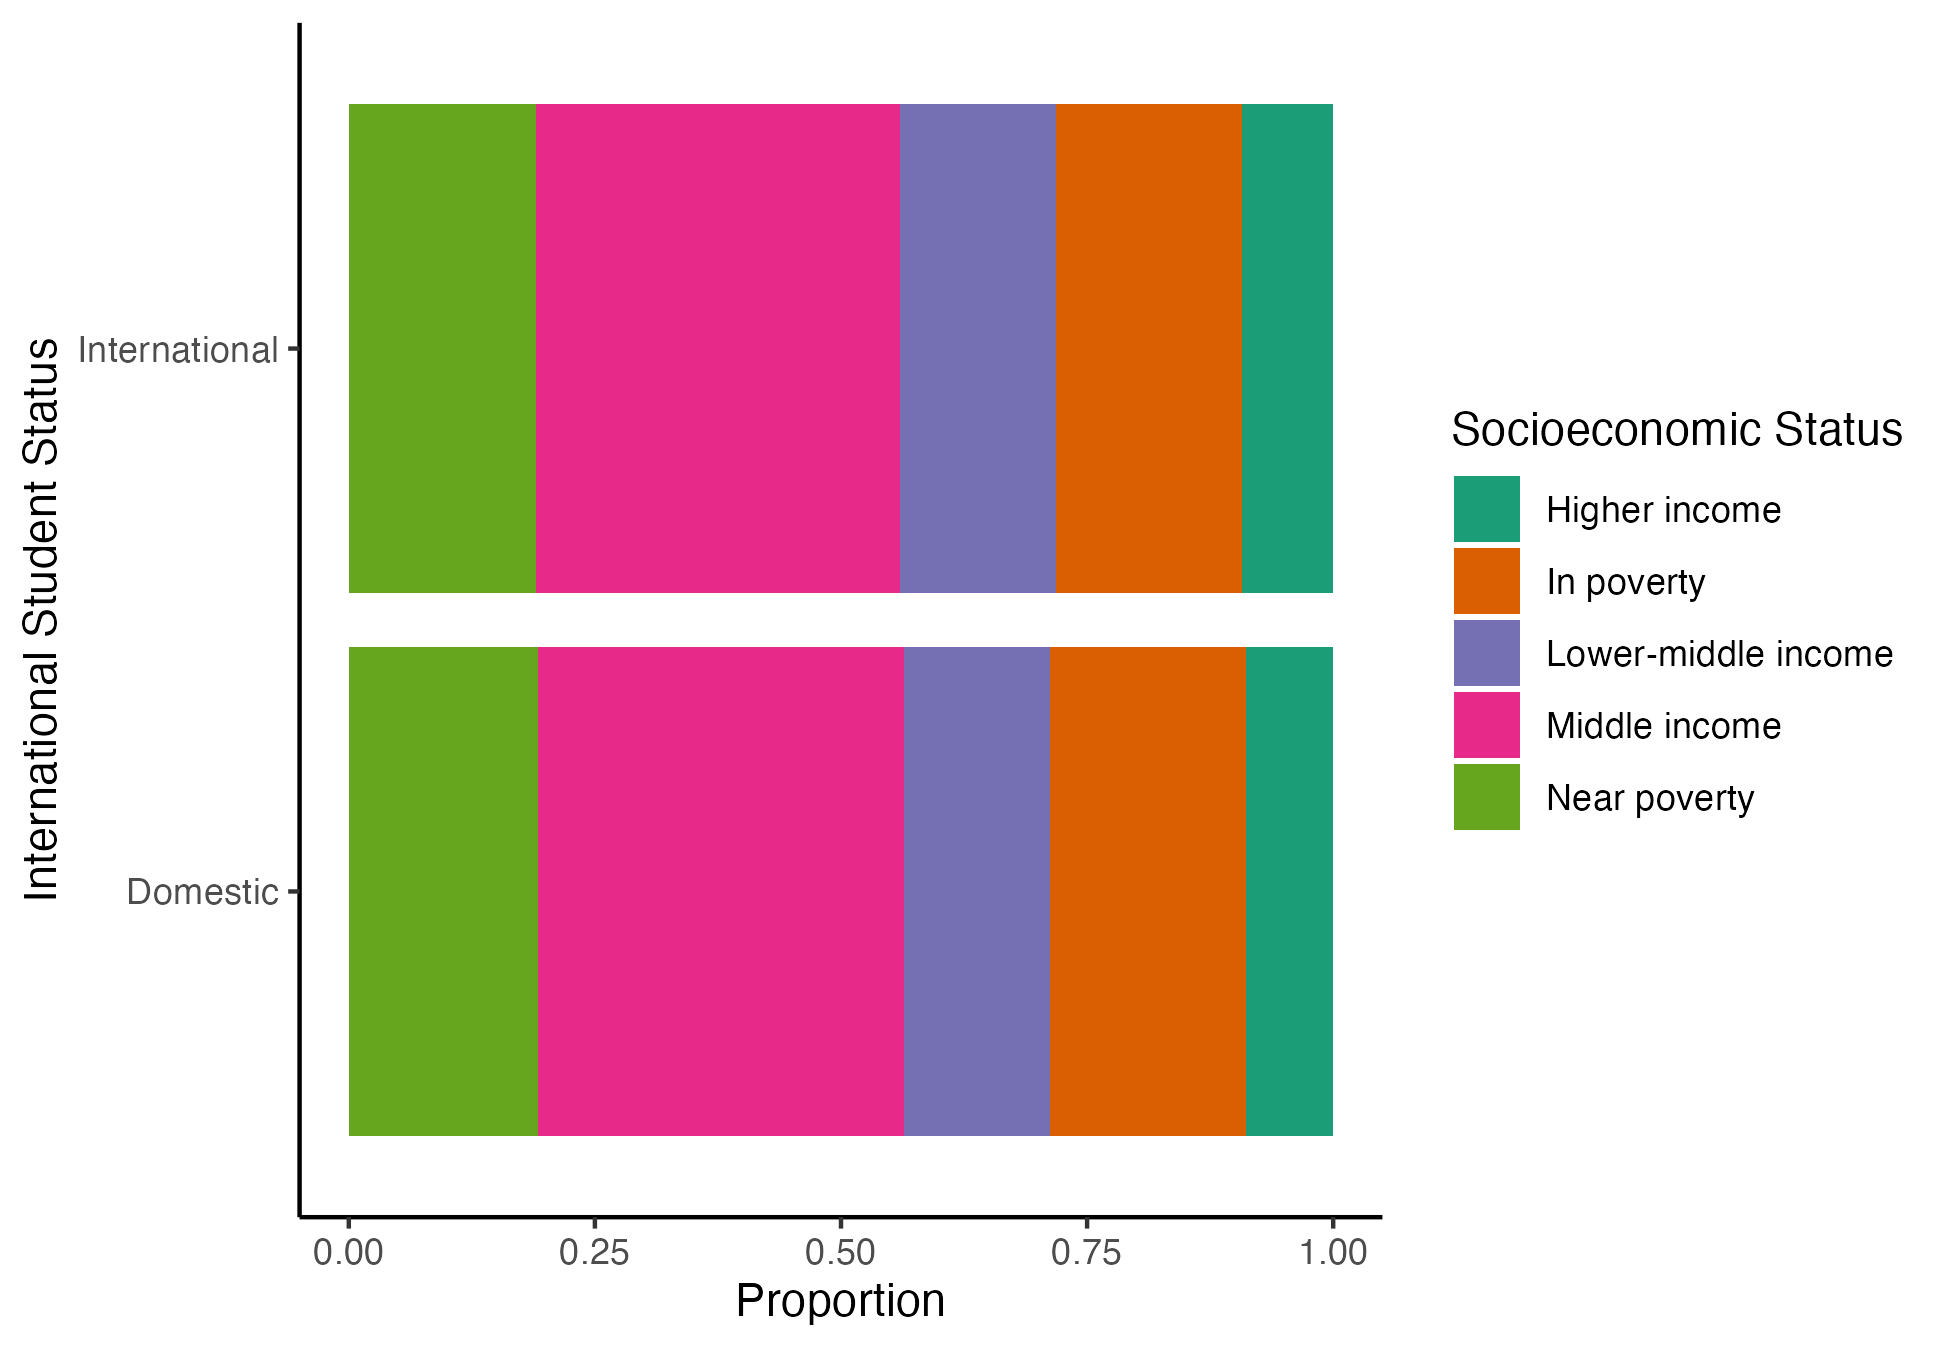
\includegraphics[width=0.9\linewidth]{international_student_status_v_socioeconomic_status} 

}

\caption{Correlation graph between international student status and socioeconomic status.}\label{fig:demg5}
\end{figure}

\subsubsection{Numerical Graphs}\label{numerical-graphs}

The graphs were generated using ggplot2 (Wickham, 2023) and use a theme from hrbrthemes (Rudis, 2024).

The gpa distribution graph (Figure \ref{fig:gpagraph}) shows the number of students with each GPA and we see how similar the distribution is to the horizontal line which represents a uniform distribution.



\begin{figure}

{\centering 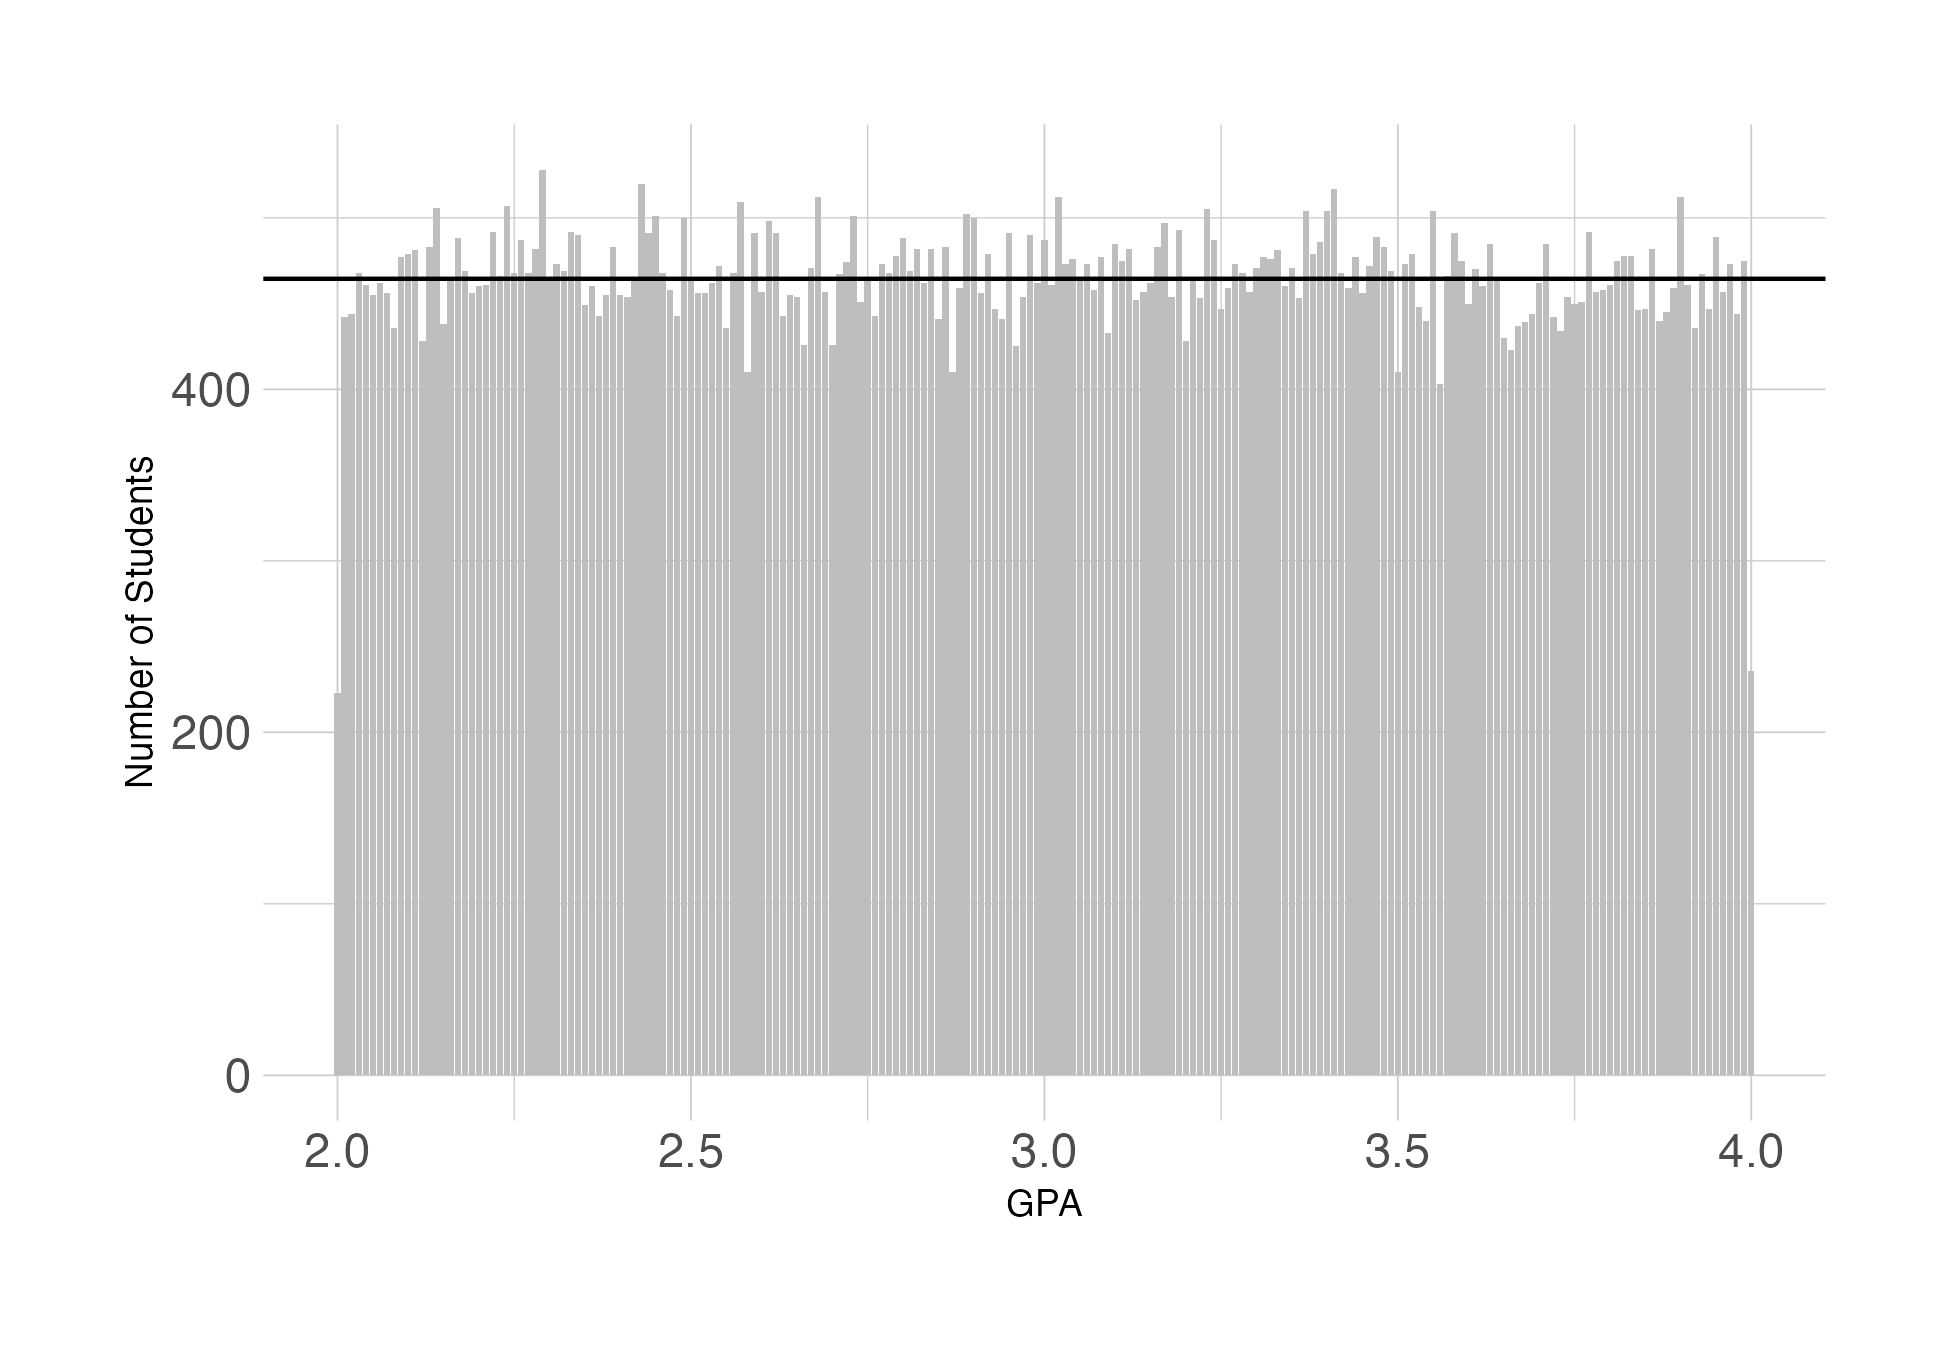
\includegraphics[width=0.9\linewidth]{gpa} 

}

\caption{Number of students with different GPAs. The horizontal gray line (y=464.4527) represents the expected values based on a uniform distribution.}\label{fig:gpagraph}
\end{figure}

The student semester distribution graph (Figure \ref{fig:studentsemestergraph}) shows the number of students in each semester and we see how similar the distribution is to the horizontal line which represents a uniform distribution.



\begin{figure}

{\centering 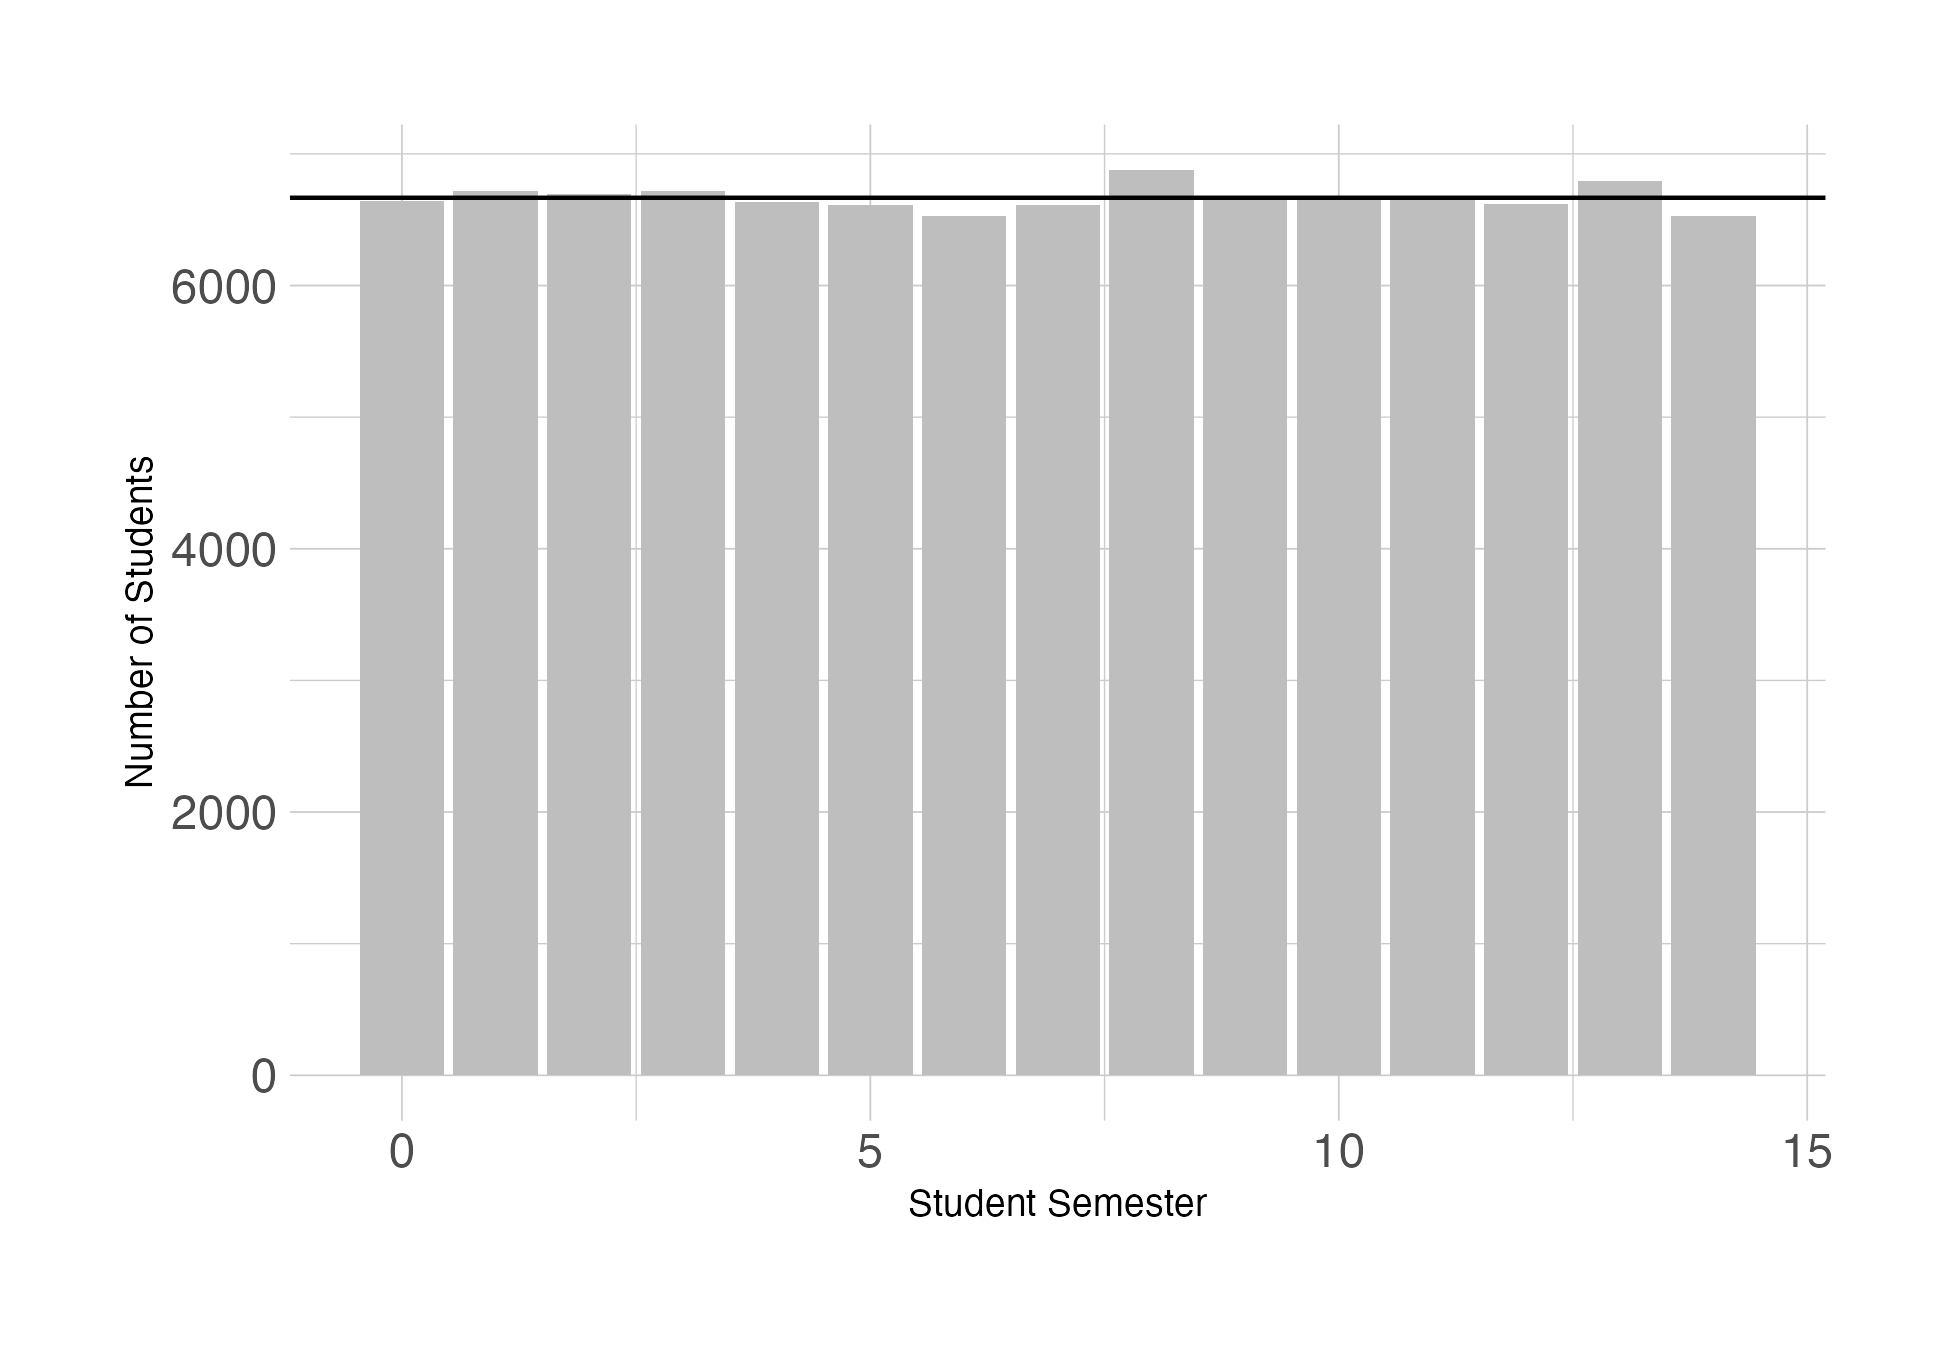
\includegraphics[width=0.9\linewidth]{student_semester} 

}

\caption{Number of students in each semester. The horizontal gray line (y=6666.667) represents the expected values based on a uniform distribution.}\label{fig:studentsemestergraph}
\end{figure}

\subsection{Major}\label{major-1}

\label{sec:major_res}

First, we discuss the popularity of each major. Then, we cover the correlations between \textbf{Major(s)} and different demographics. Finally, we graph various distributions of major choice depending on gender identity.

\subsubsection{Major Popularity}\label{major-popularity}

Figure \ref{fig:topmajorgraph} shows the top ten most popular majors in the \emph{Purely Synthetic Educational Dataset}.



\begin{figure}

{\centering 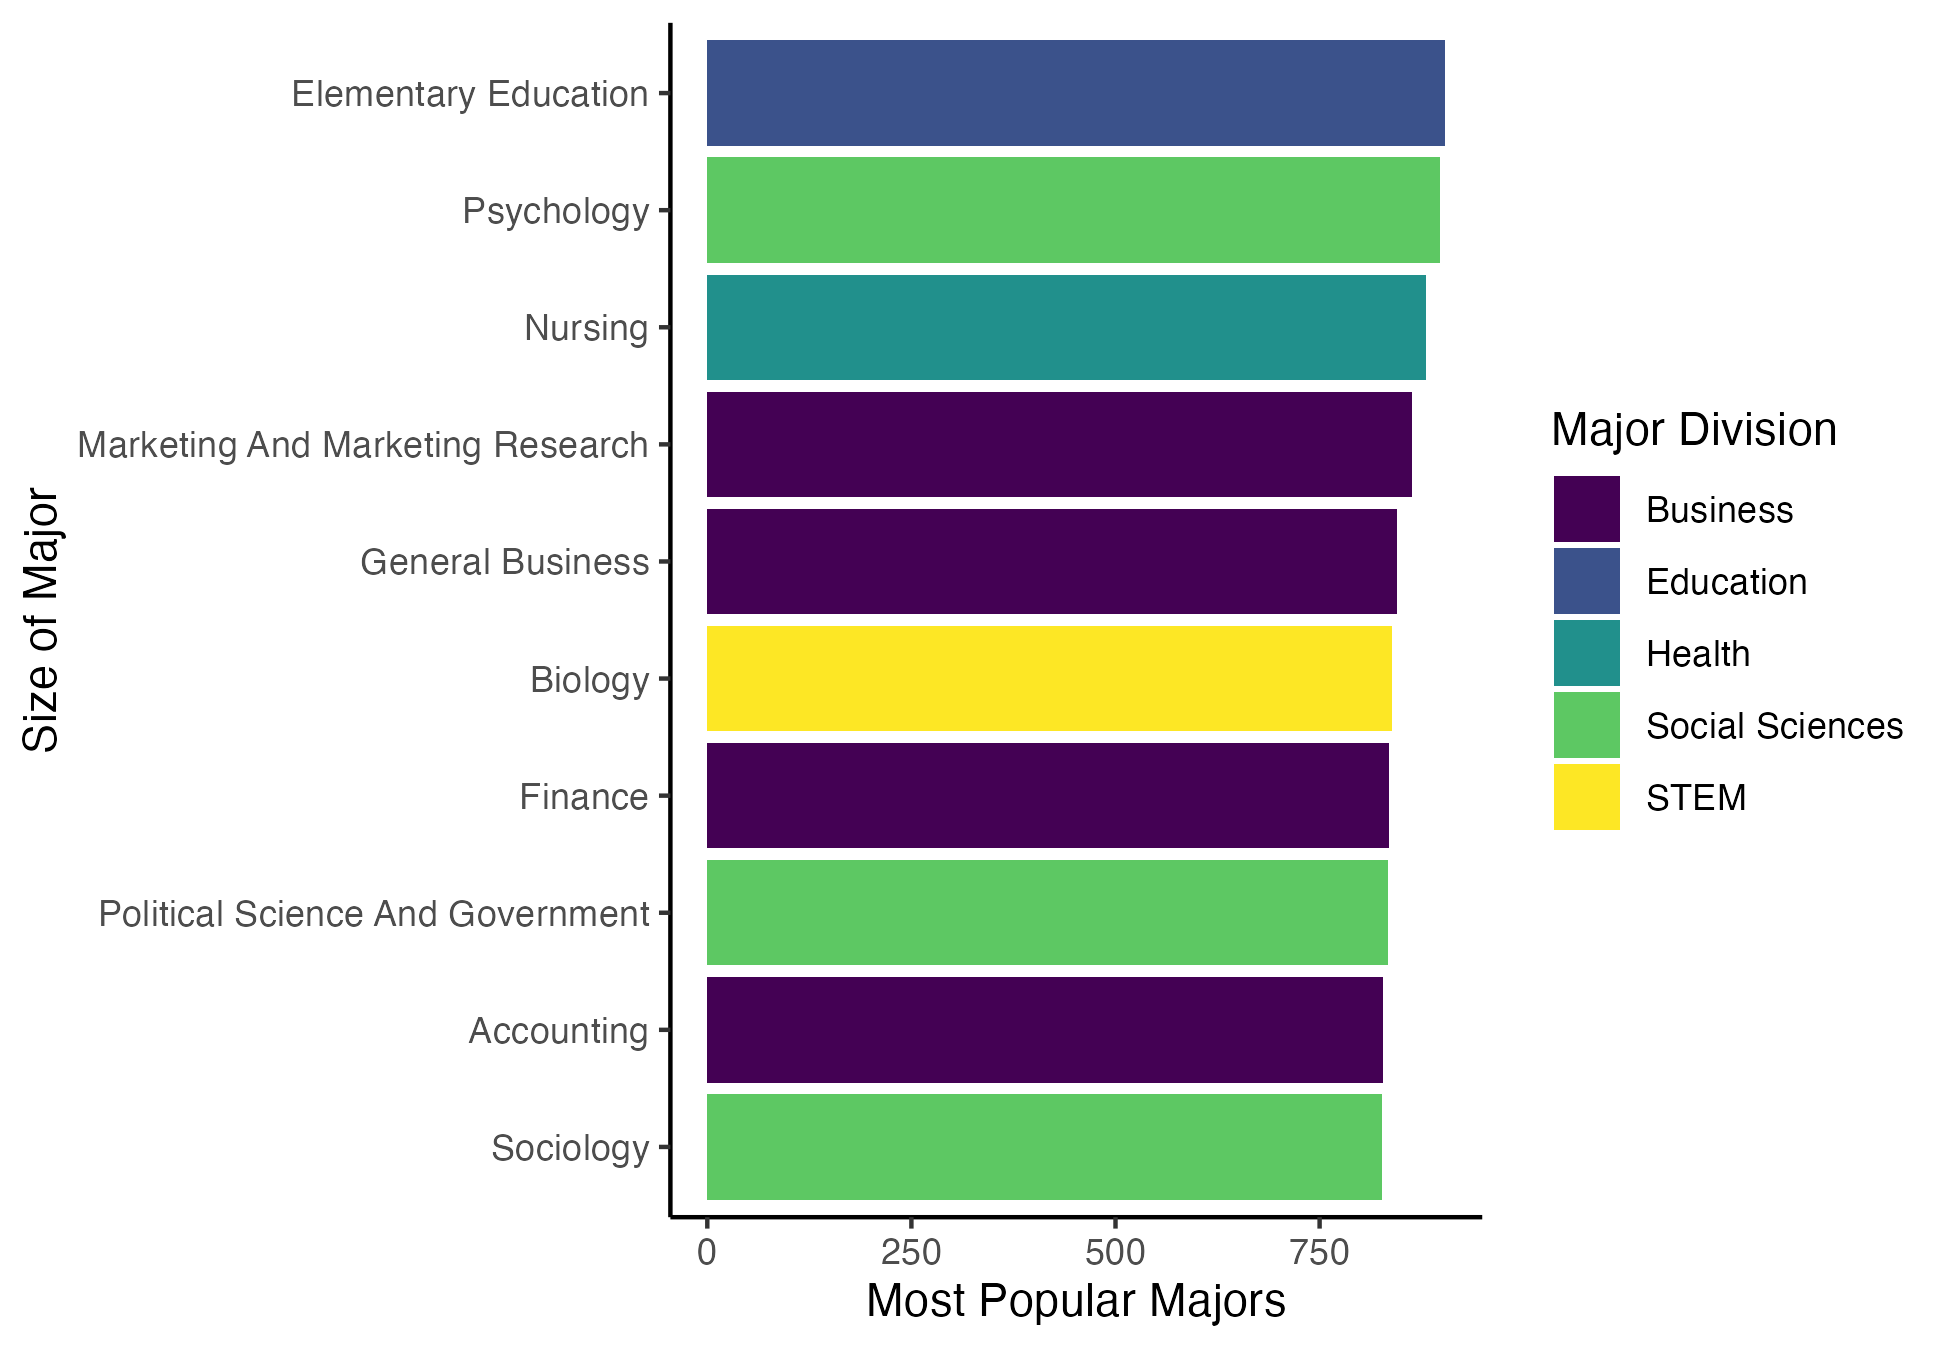
\includegraphics[width=0.9\linewidth]{top_major_graph} 

}

\caption{Top 10 majors by popularity organized by division.}\label{fig:topmajorgraph}
\end{figure}

Figure \ref{fig:obsvsexptopmajorsgraph} shows the majors comparing their observed and expected popularity. The Chi Squared Goodness of Fit Test between the expected and observed major popularity gave a p-value of \(<2.2e^{-16}\).



\begin{figure}

{\centering 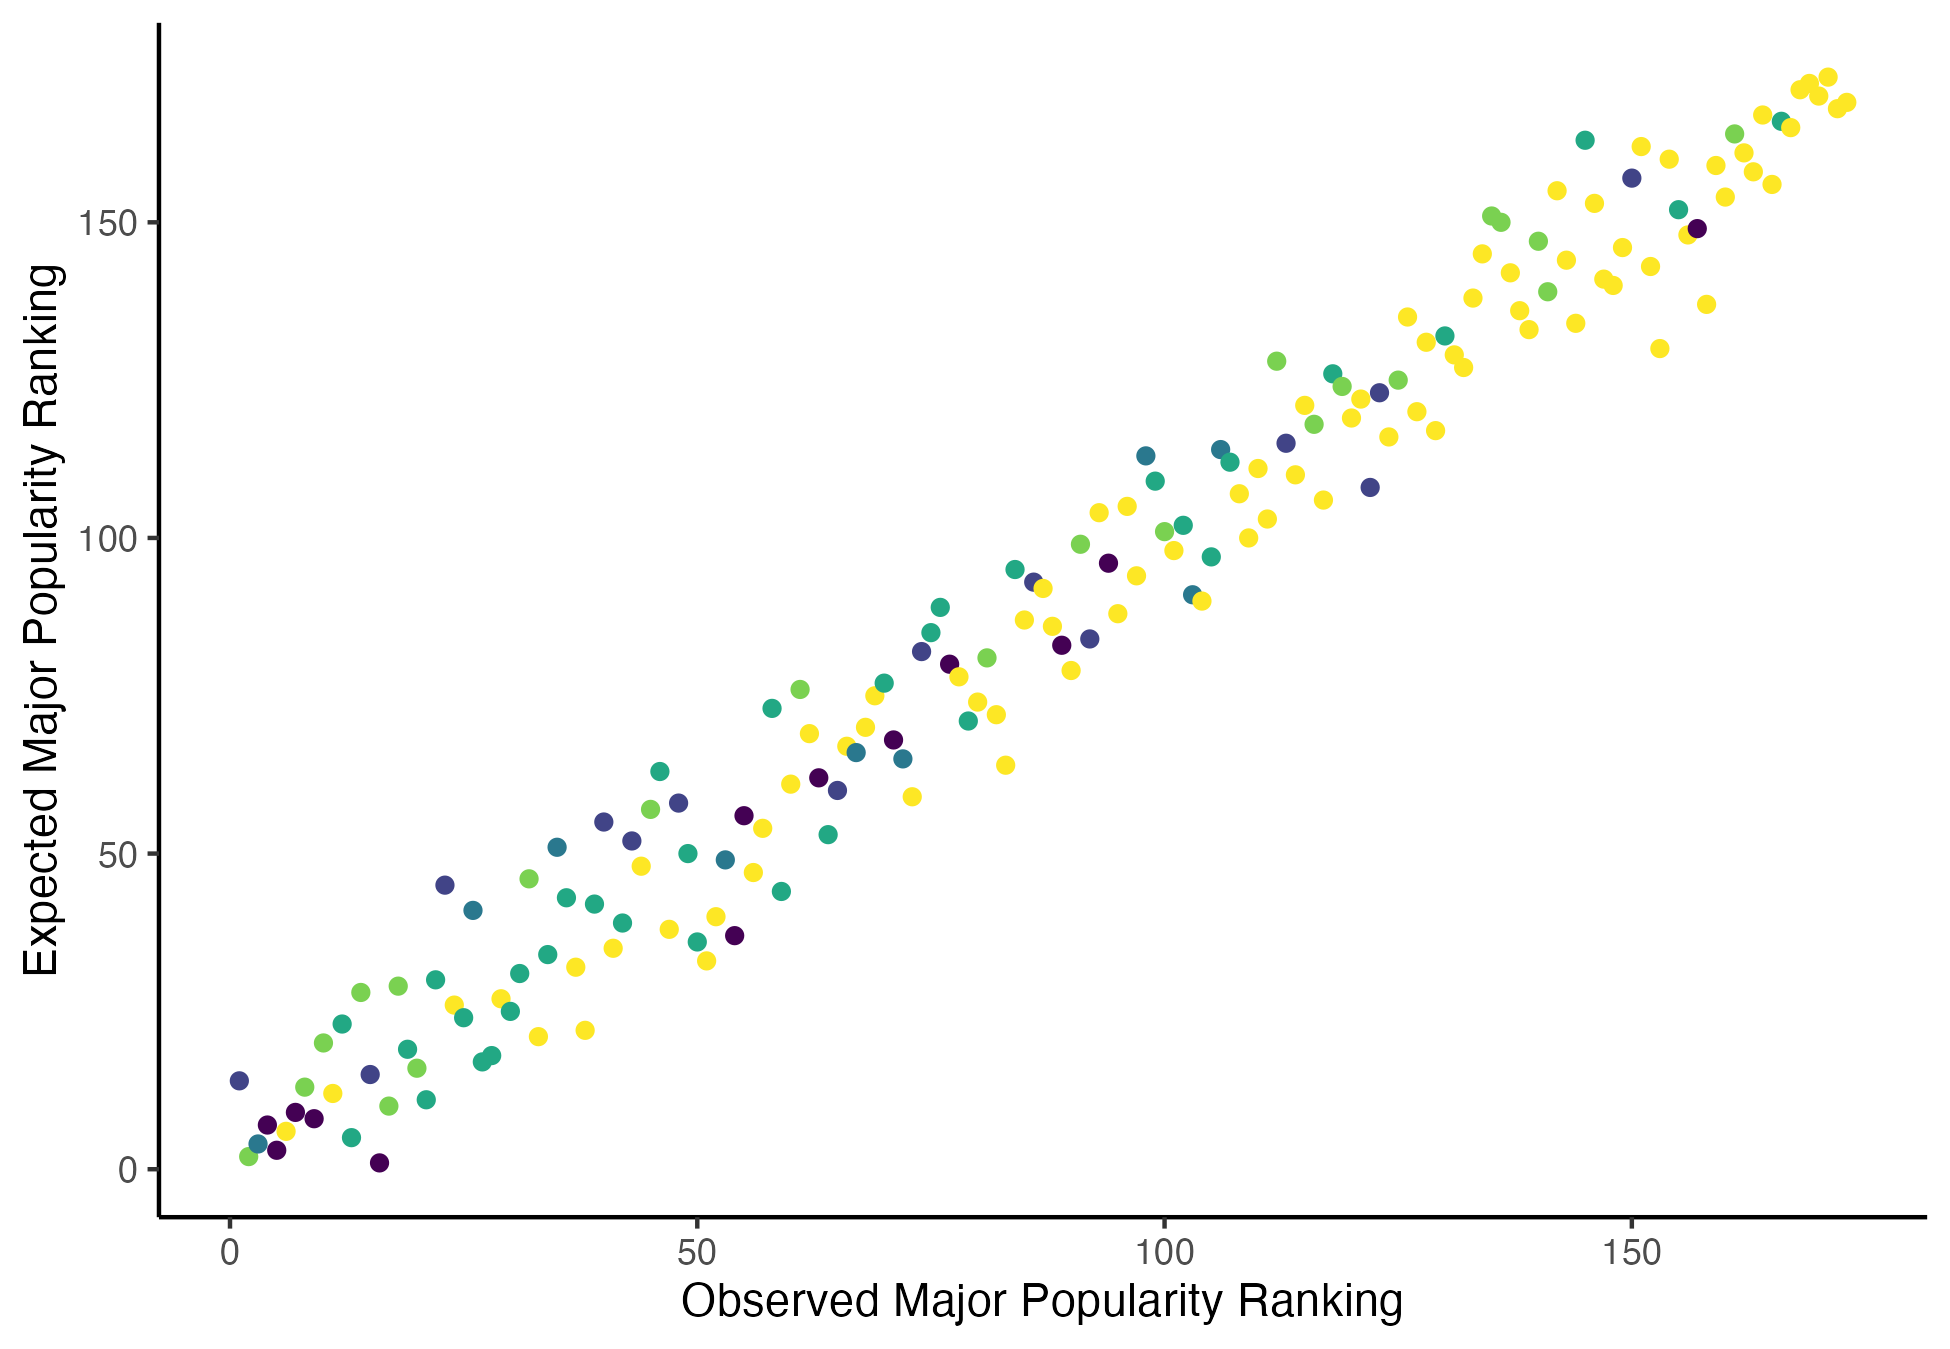
\includegraphics[width=0.9\linewidth]{obs_vs_exp_majors} 

}

\caption{Observed vs expected major popularity organized by division.}\label{fig:obsvsexptopmajorsgraph}
\end{figure}

\subsubsection{Major Correlations}\label{major-correlations}

Table \ref{tab:major_chi_indep} shows the correlations between \textbf{Major(s)} and several demographics. Only \textbf{Gender} is not independent of the \textbf{Major(s)} features.

\begin{table}[htbp]
  \centering
  \begin{tabular}{|l|l|l|}
    \hline
    \textbf{Demographic} & \textbf{Major Correlation} & \textbf{Division Correlation} \\ \hline
    Ethnoracial Group & 0.8966 & 0.1593 \\ \hline
    Gender & $<2.2e^{-16}*$ & $<2.2e^{-16}*$ \\ \hline
    International Student Status & 0.7619 & 0.2205 \\ \hline
    Socioeconomic Status & 0.7008 & 0.3414 \\ \hline
  \end{tabular}
  \caption{Chi Squared Test of Independence between Major and the demographics. *p<0.05}
  \label{tab:major_chi_indep}
\end{table}

\subsubsection{Gender by Major}\label{gender-by-major-1}

Figure \ref{fig:expvsobsgxm} shows the expected and observed percent of female identifying students in each major. The observed (dark gray line) and expected (light gray line) linear regression are visually dissimilar. The Chi Squared Goodness of Fit Test between the expected and observed percent of female identifying students gave a p-value of 1.



\begin{figure}

{\centering 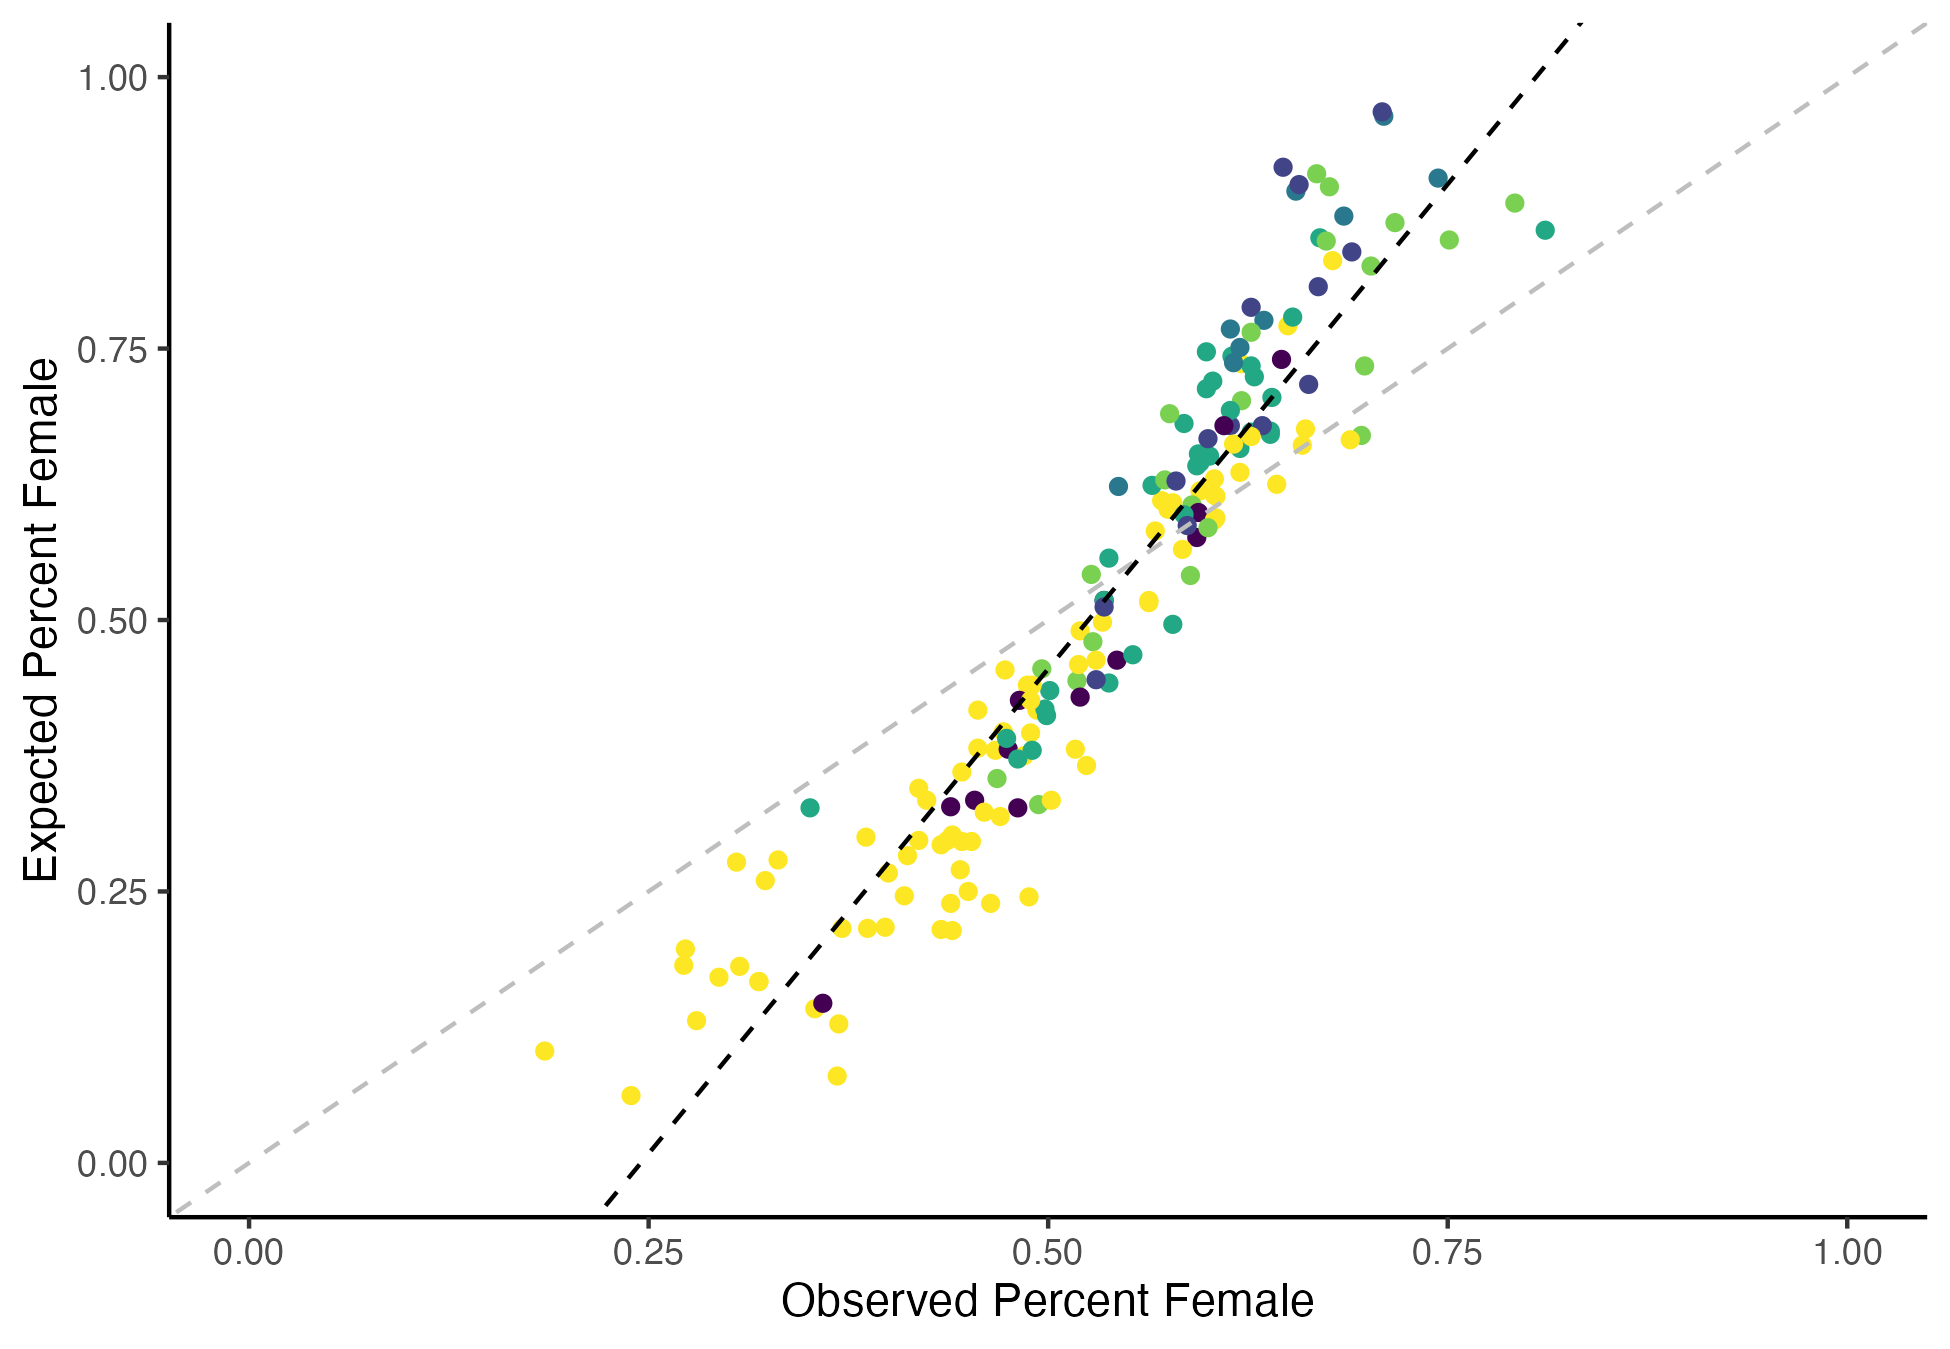
\includegraphics[width=0.9\linewidth]{obs_vs_exp_gxm} 

}

\caption{Expected vs observed percent female per major, colored by division. The dark gray line (y=1.7855x-0.4378) is the linear regression. The light gray line (y=x) is the expected linear regression, since expected and observed.}\label{fig:expvsobsgxm}
\end{figure}

Figure \ref{fig:expvsobsgxm} shows the expected and observed percent of female identifying students in each major. This graph was interactive in the HTML, but that does not work in pdf and so the circles mostly cover each other since the size represents the number of students in each major.



\begin{figure}

{\centering 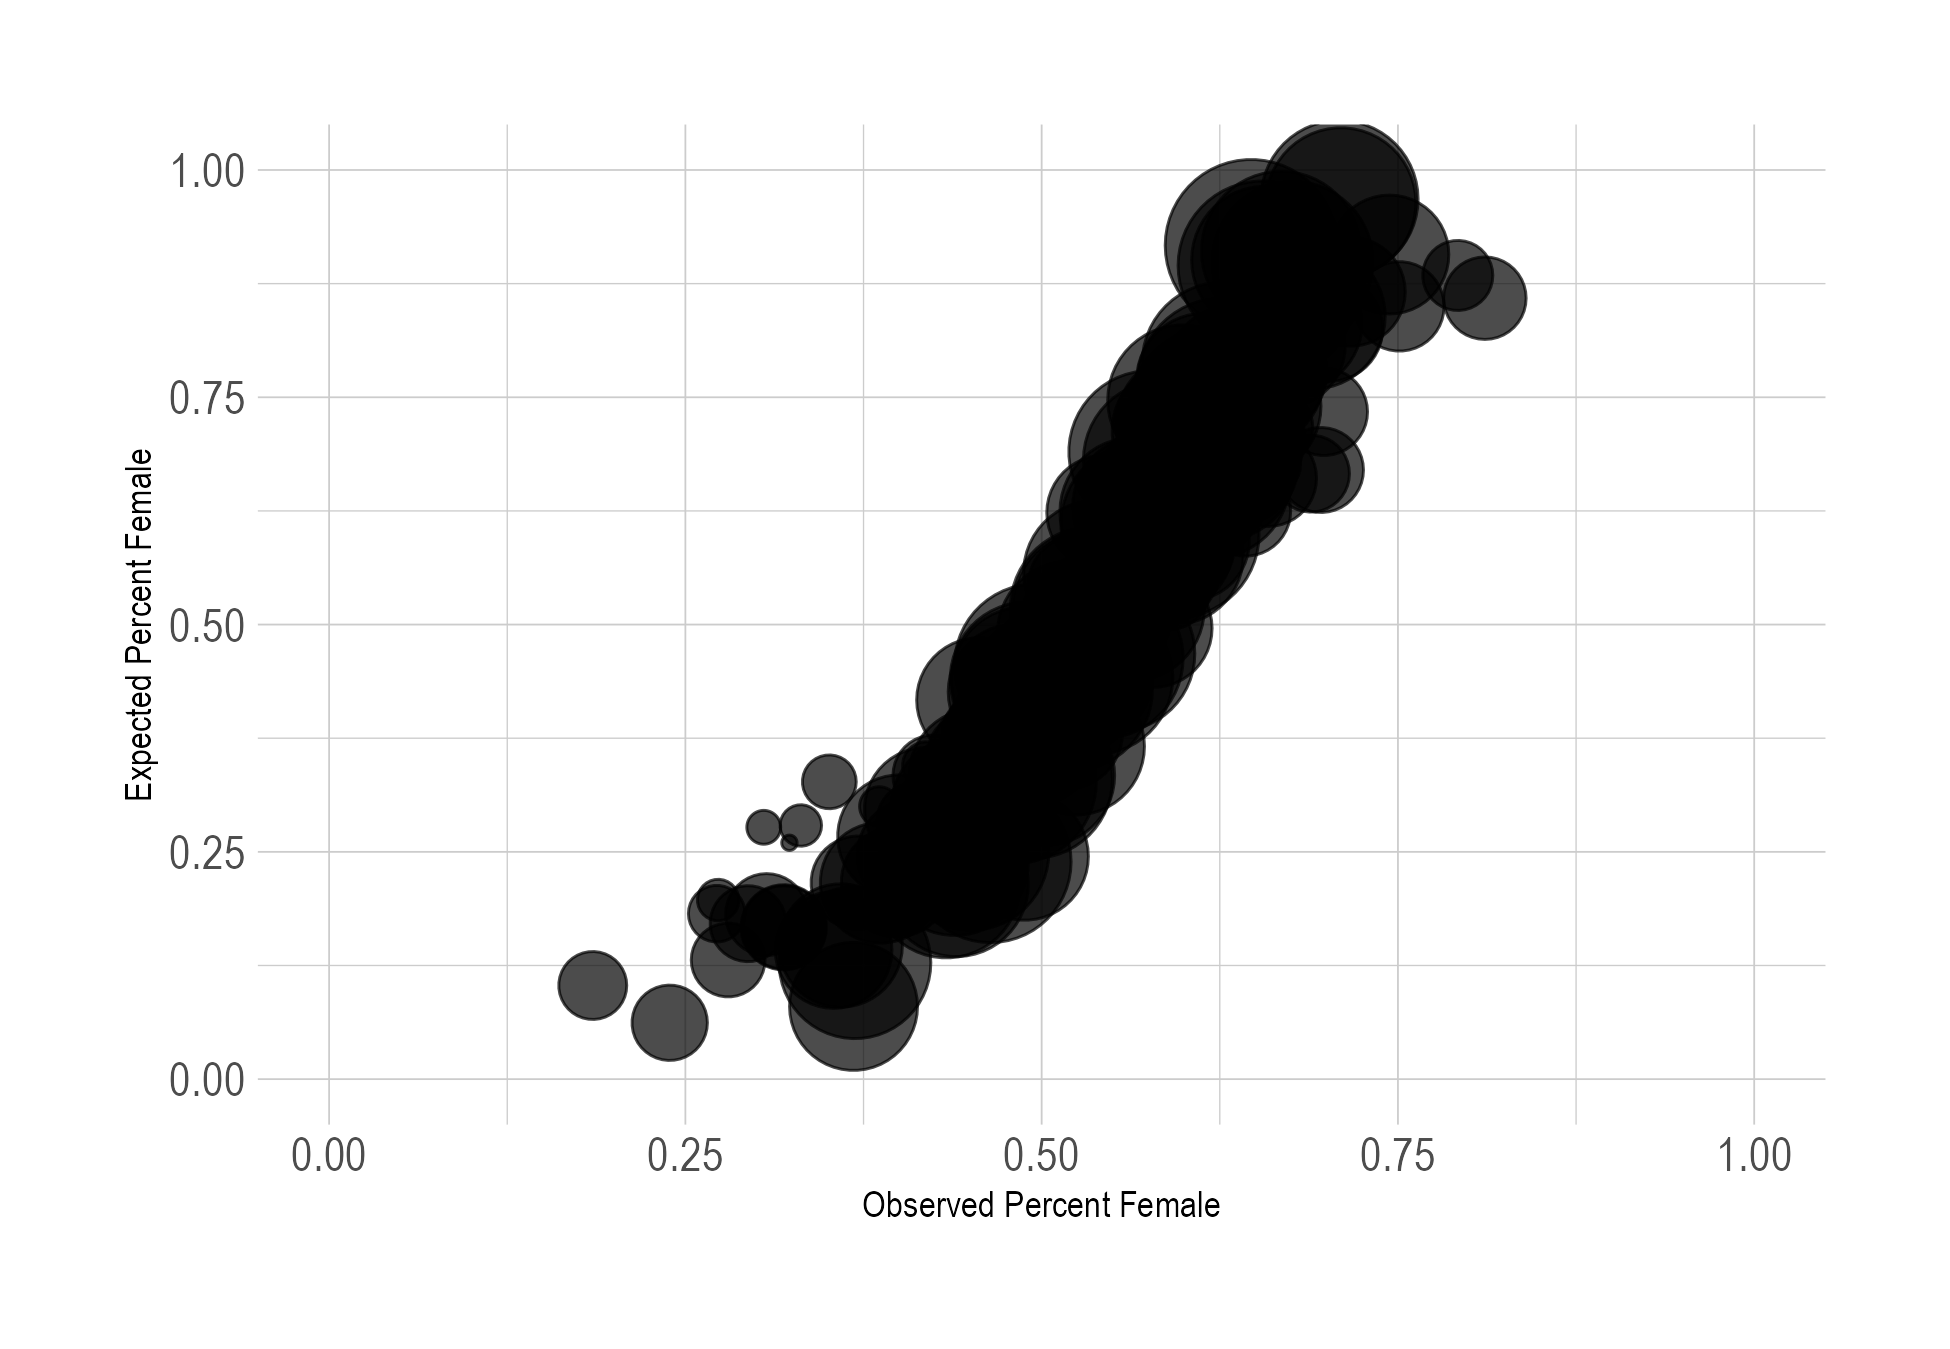
\includegraphics[width=0.9\linewidth]{obs_vs_exp_gxm_major_size} 

}

\caption{Observed vs expected percent female by major. Circles are the number of majors. In the HTML this was colored by Major Division and an interactive graph, but that does not work with a pdf output.}\label{fig:obsvsexpmajorsizegraph}
\end{figure}

Figure \ref{fig:maledomgraph} shows the top ten majors that are dominated by male identifying students. All these majors are in the STEM division.



\begin{figure}

{\centering 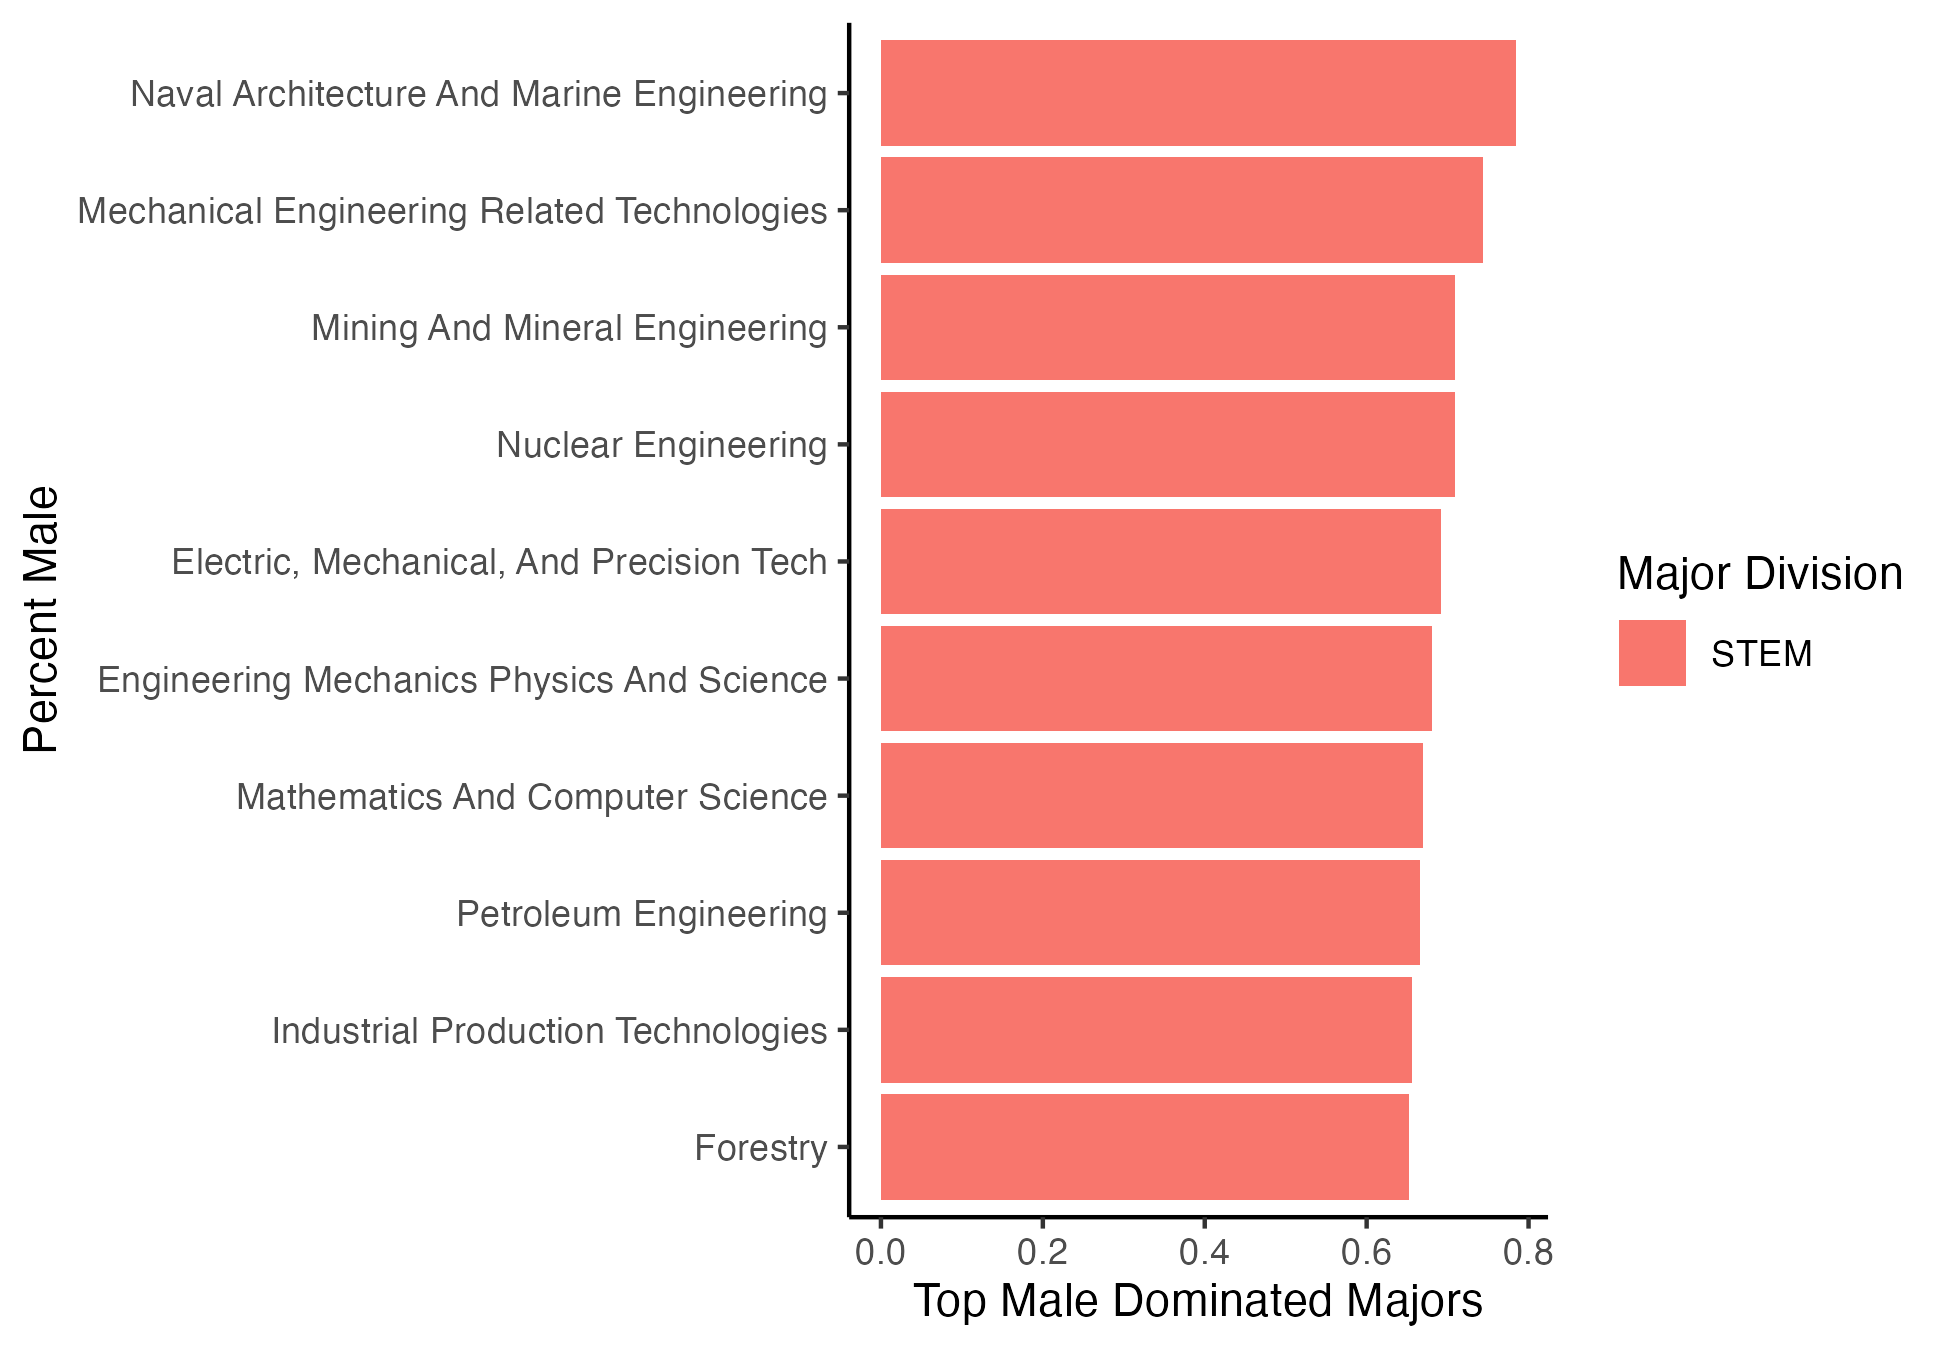
\includegraphics[width=0.9\linewidth]{male_dom} 

}

\caption{Top ten majors with the highest percentage of male students. Colored by division.}\label{fig:maledomgraph}
\end{figure}

Figure \ref{fig:femaledomgraph} shows the top ten majors that are dominated by female identifying students. The majors are from a variety of divisions.



\begin{figure}

{\centering 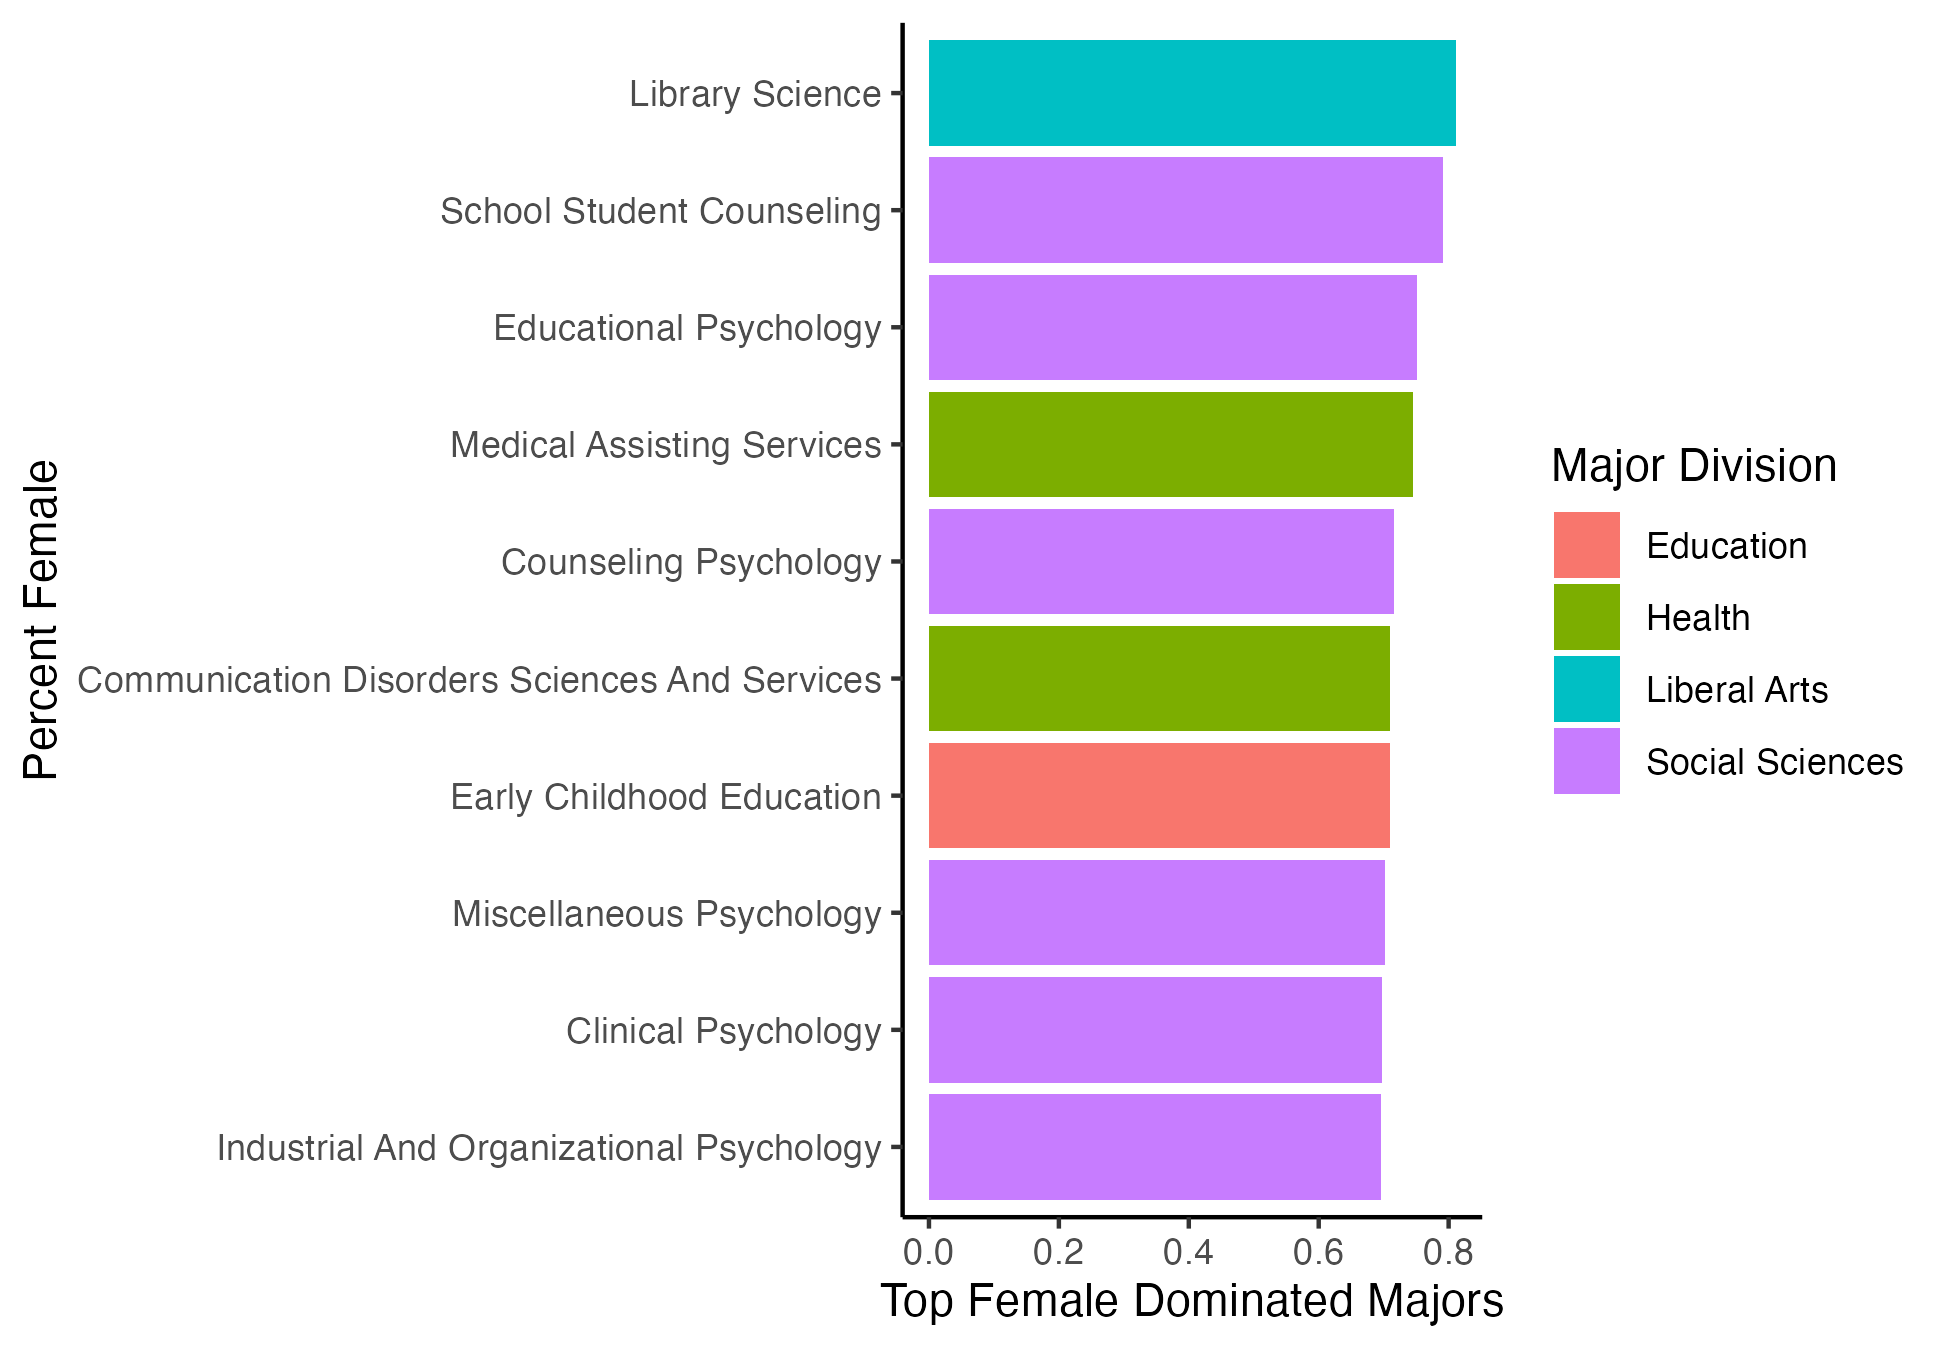
\includegraphics[width=0.9\linewidth]{female_dom} 

}

\caption{Top ten majors with the highest percentage of female students. Colored by division.}\label{fig:femaledomgraph}
\end{figure}

Figure \ref{fig:genmindomgraph} shows the top ten majors that are dominated by gender minority (female and nonbinary) students. The majors are from a variety of divisions.



\begin{figure}

{\centering 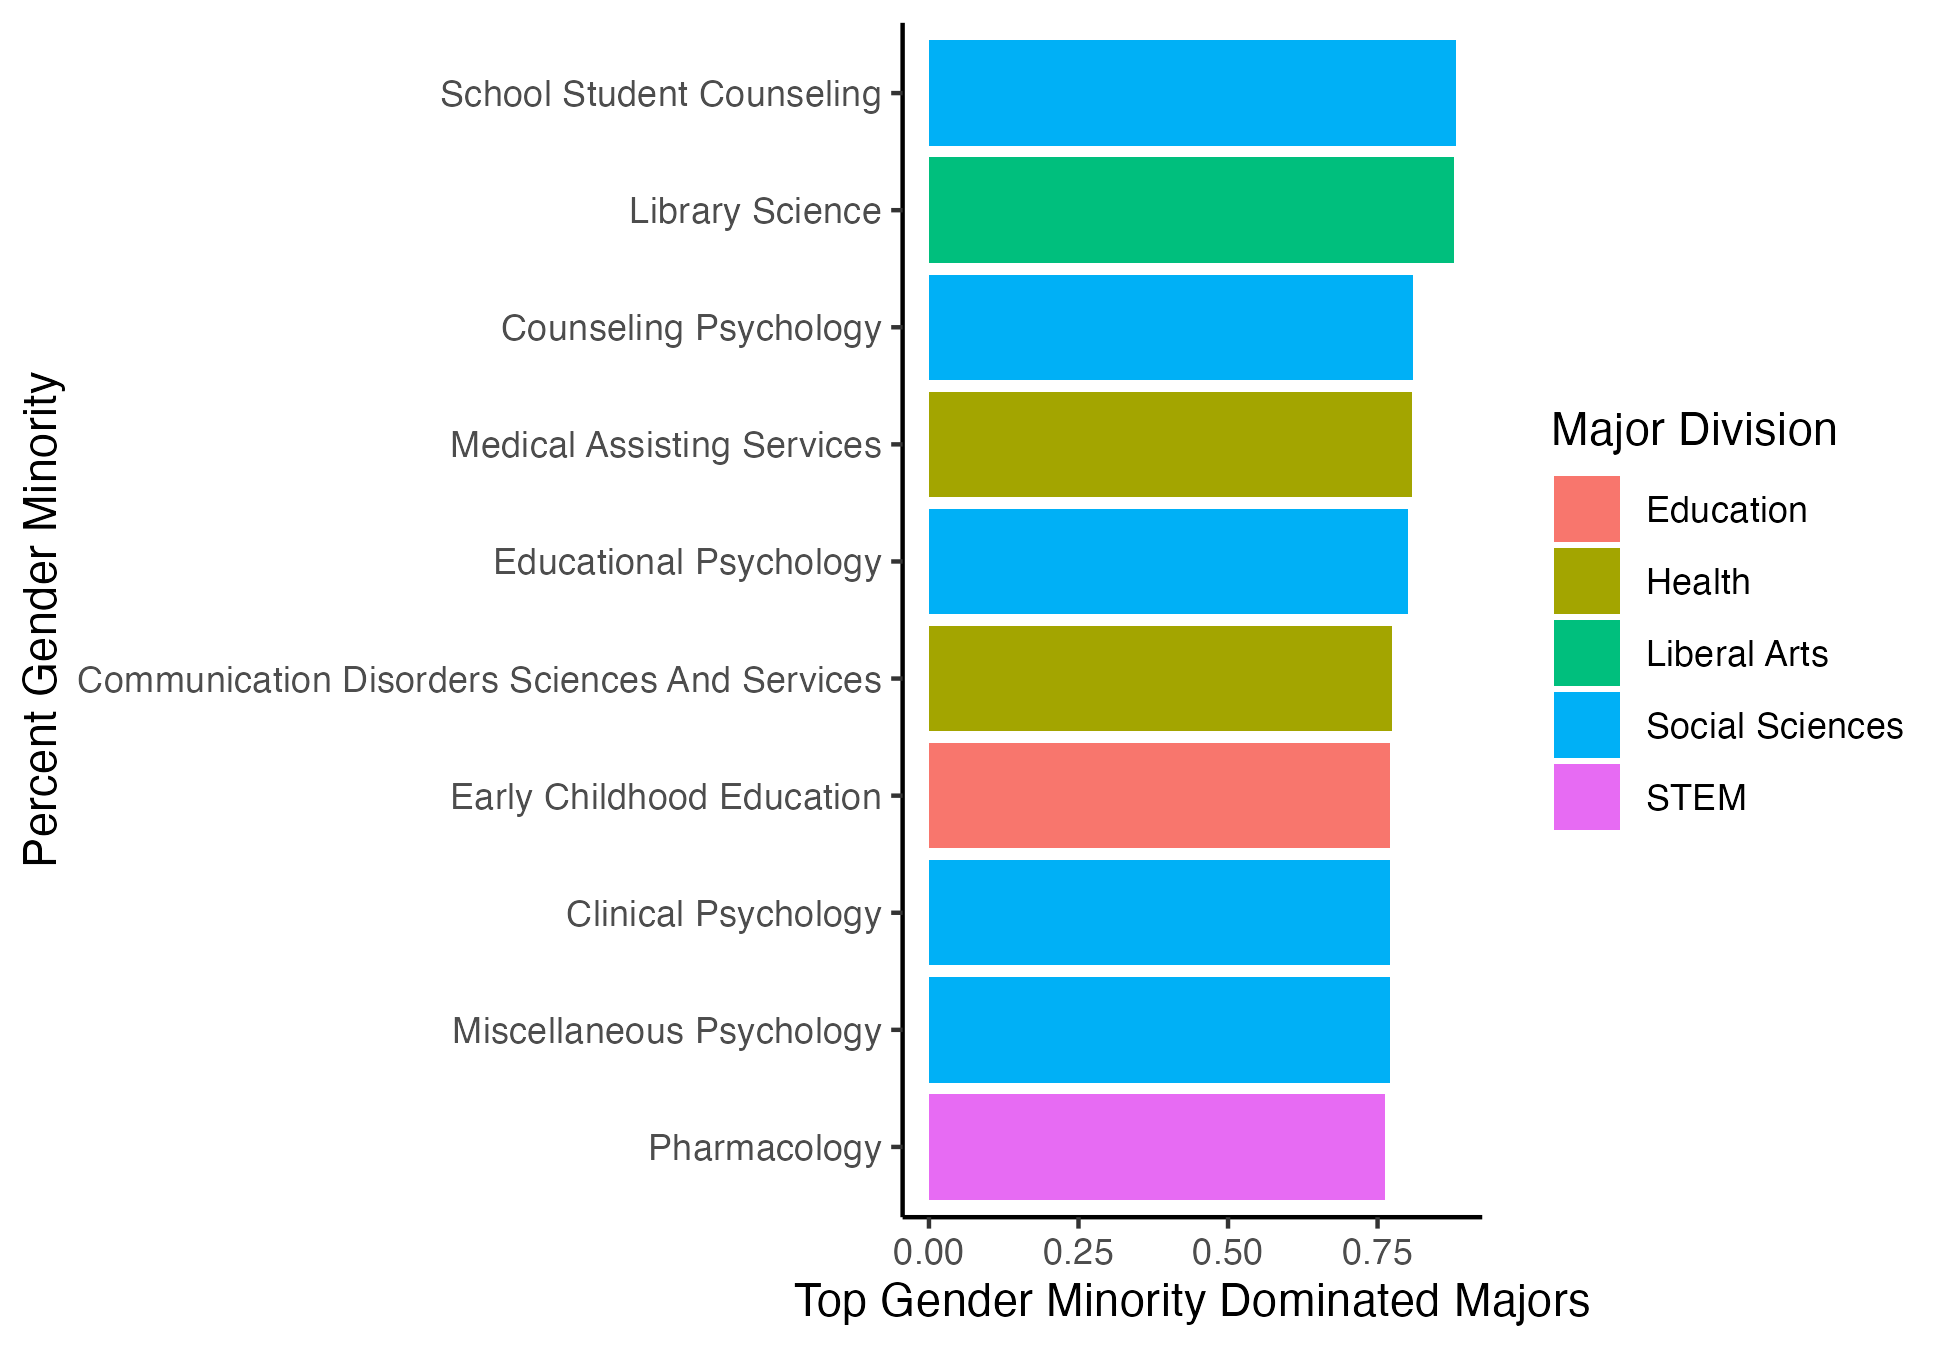
\includegraphics[width=0.9\linewidth]{gen_min_dom} 

}

\caption{Top ten majors with the highest percentage of male students. Colored by division.}\label{fig:genmindomgraph}
\end{figure}

No graph was made of nonbinary students, since there are not enough nonbinary students for any major to be majority nonbinary.

\subsection{Learning Style}\label{learning-style-1}

\label{sec:learning_style_res}

Table \ref{tab:learning_style_chi_indep} shows the correlations between \textbf{Learning Style(s)} and the demographic features. None of them are significant, so they are all independent.

\begin{table}[htbp]
  \centering
  \begin{tabular}{|l|l|}
    \hline
    \textbf{Demographic} & \textbf{Learning Style Correlation} \\ \hline
    Ethnoracial Group & 0.4939 \\ \hline
    Gender & 0.98 \\ \hline
    International Student Status & 0.6115 \\ \hline
    Socioeconomic Status & 0.6034 \\ \hline
  \end{tabular}
  \caption{Chi Squared Test of Independence between Learning Style and the demographics. *p<0.05}
  \label{tab:learning_style_chi_indep}
\end{table}

\subsection{Complex Correlations}\label{complex-correlations-1}

\label{sec:complex_correlations_res}

Table \ref{tab:complex_chi_indep} shows the correlations between \textbf{Major(s)} and \textbf{Previous Course Subjects} as well as \textbf{Learning Style(s)} and \textbf{Previous Course Types}. The test between \textbf{Major(s)} and \textbf{Previous Course Subjects} was significant and so they are correlated. However, the test between \textbf{Learning Style(s)} and \textbf{Previous Course Types} was not significant, so they are independent.

\begin{table}[htbp]
  \centering
  \begin{tabular}{|l|l|}
    \hline
    \textbf{Comparison} & \textbf{Correlation} \\ \hline
    Major vs Previous Course Subjects & $<2.2e^{-16}*$ \\ \hline
    Learning Style vs Previous Course Types & 0.9967 \\ \hline
  \end{tabular}
  \caption{Chi Squared Test of Independence. *p<0.05}
  \label{tab:complex_chi_indep}
\end{table}

\section{Discussion}\label{discussion}

In this section we discuss each of the results sections and consider challenges and obstacles. Then we return to the hypothesis and the predictions and finish with the future work section.

\begin{enumerate}
\def\labelenumi{\arabic{enumi}.}
\tightlist
\item
  Demographics (\ref{sec:demographics_dis})
\item
  Major (\ref{sec:major_dis})
\item
  Learning Style (\ref{sec:learning_style_dis})
\item
  Obstacles and Challenges (\ref{sec:obstacles_challenges})
\item
  Hypothesis and Predictions (\ref{sec:hypothesis_predictions})
\item
  Future Work (\ref{sec:future_work})
\end{enumerate}

\subsection{Demographics}\label{demographics-2}

\label{sec:demographics_dis}

The extremely high p-values from the Chi Squared Goodness of Fit Test show that \textbf{Ethnoracial Group}, \textbf{Gender}, \textbf{International Student Status}, and \textbf{Socioeconomic Status} all closely math the empirical sampling distribution taken from Nicolas \& Sakib (2024). Visually, we see that \textbf{GPA} and \textbf{Student Semester} match the uniform distribution from which they were sampled.

The insignificant p-values from the Chi Squared Test of Independence show that \textbf{Ethnoracial Group}, \textbf{Gender}, \textbf{International Student Status}, and \textbf{Socioeconomic Status} are independent and not correlated with eachother. Notably there is high variation in the p-values with \textbf{Ethnoracial Group} and \textbf{Gender} having a very high p-value (0.8605), while \textbf{International Student Status}, and \textbf{Socioeconomic Status} have an almost significant p-value (0.08951).

\subsection{Major}\label{major-2}

\label{sec:major_dis}

The extremely high p-value from the Chi Squared Goodness of Fit Test show that gender distribution among \textbf{Major(s)} closely matches the empirical data used in the weighting function. However, the extremely low p-value from the Chi Squared Goodness of Fit Test show that major popularity within \textbf{Major(s)} does not match the empirical data used in the weighting function. Thus, the weighting function generated by Nicolas \& Sakib (2024) does not properly weight the majors to reflect the empirical data.

The insignificant p-values from the Chi Squared Test of Independence show that \textbf{Ethnoracial Group}, \textbf{International Student Status}, and \textbf{Socioeconomic Status} are independent from and not correlated with \textbf{Major(s)}. This was expected since none of these variables are explicitly mapped to \textbf{Major(s)}. The very low p-values from the Chi Squared Test of Independence show that \textbf{Gender} and \textbf{Previous Course Subjects} are correlated with \textbf{Major(s)}. This was expected since \textbf{Gender} is explicitly mapped to \textbf{Major(s)} which is explicitly mapped to \textbf{Previous Courses}.

Looking at the top ten majors dominated by different gender identities, we see that all the male dominated majors are STEM while the female or gender minority dominated majors come from a variety of divisions. Looking at Figure \ref{fig:expvsobsgxm} we see that for majors with few female students more female students were observed than expected. At the same time, for majors with more female students less female students were observed than expected. Since some randomization was used in the majors function (Nicolas \& Sakib, 2024), perhaps this had a normalizing effect which is why only majors at the extremities (very high or very low percentage of female students) were pushed closer to being even balanced between genders (around 50\% female).

\subsection{Learning Style}\label{learning-style-2}

\label{sec:learning_style_dis}

The extremely high p-value from the Chi Squared Goodness of Fit Test show that \textbf{Learning Style(s)} all closely math the empirical sampling distribution taken from Nicolas \& Sakib (2024). The insignificant p-values from the Chi Squared Test of Independence show that \textbf{Ethnoracial Group}, \textbf{Gender}, \textbf{International Student Status}, \textbf{Socioeconomic Status}, and \textbf{Previous Course Types} are independent and not correlated with \textbf{Learning Style(s)}. This was unexpected since \textbf{Learning Style(s)} was explicitly mapped to \textbf{Previous Course Types}.

\subsection{Obstacles and Challenges}\label{obstacles-and-challenges}

\label{sec:obstacles_challenges}

Since the list features in the \emph{Purely Synthetic Educational Dataset} were imported as strings, once they were split and recombined the dataset became very large (\textgreater1,000,000 rows). This limited the tables and graphs that could be made with these features. This is why only the list features \textbf{Major(s)} and \textbf{Learning Style(s)} which have at most 2 entries were examined closely as they never made the dataset larger than 200,000 rows. Another difficulty was how many of the graphics were made to be interactive and while this worked when knitted to HTML, knitting to pdf prevented interactive graphics. Thus, the graphs shown here are slightly altered versions of the interactive HTML graphics. Finally, the extremely large size of the dataset (100,000 rows and 17 columns) meant that not all features could be examined within the time frame.

\subsection{Hypothesis and Predictions}\label{hypothesis-and-predictions}

\label{sec:hypothesis_predictions}

Now we return to our predictions and hypothesis (Table \ref{tab:hypothesis_predictions}). All of the features matched their empirical sampling distributions except for major popularity. Thus, the first prediction is mostly supported overall. For the second prediction, only three explicit mappings were measured and two of three showed correlations between the two features. The converse of the second prediction was true with all of the non explicitly mapped features being independent and not correlated with each other.

Thus, the three predictions overall do support the hypothesis that the data generation function from Nicolas \& Sakib (2024) works as intended. The nuance comes from the major weighting function, and also the independence of \textbf{Learning Style(s)} and \textbf{Previous Course Types} which were explicitly mapped.

\subsection{Future Work}\label{future-work}

\label{sec:future_work}

Repeating the same testing on the remaining variables in the dataset can further support the hypothesis and the notion that the dataset is usable for educational research. Additionally, future work should focus on attempting to fix the parts of the generating function that did not work as expected. Once, they are changed, a new dataset could be generated and then the analysis in this work could be repeated on the newly generated dataset. This work only showed that certain features were correlated, but a more advanced statistical analysis is needed to show the strength of the correlation.

Once this work is done, and the dataset has been shown to truly represent the empirical data, then the dataset can be used for educational research. Since the dataset is purely synthetic it is not connected to any real people, and thus poses no privacy risk. Previous educational research (Guan et al., 2020; Shao et al., 2021) can be redone with the purely synthetic educational dataset to further test the effectiveness of the dataset at replacing empirical data or synthetic data that is based in empirical data.

\section*{References}\label{references}
\addcontentsline{toc}{section}{References}

\phantomsection\label{refs}
\begin{CSLReferences}{1}{0}
\bibitem[\citeproctext]{ref-asai2020}
Asai, S. (2020). \emph{Dict: {R6 Based Key-Value Dictionary Implementation}}.

\bibitem[\citeproctext]{ref-zotero-106}
College {Majors Explorer}. (n.d.). In \emph{Big Economics}. https://bigeconomics.org/college-majors-explorer/.

\bibitem[\citeproctext]{ref-garnier2024}
Garnier, S., Ross, N., Rudis, B., Sciaini, M., Camargo, A. P., \& Scherer, C. (2024). \emph{Viridis: {Colorblind-Friendly Color Maps} for {R}}.

\bibitem[\citeproctext]{ref-gonsior2021}
Gonsior, J., Thiele, M., \& Lehner, W. (2021). \emph{{ImitAL}: {Learning Active Learning Strategies} from {Synthetic Data}} (arXiv:2108.07670). arXiv. \url{https://doi.org/10.48550/arXiv.2108.07670}

\bibitem[\citeproctext]{ref-guan2020}
Guan, C., Mou, J., \& Jiang, Z. (2020). Artificial intelligence innovation in education: {A} twenty-year data-driven historical analysis. \emph{International Journal of Innovation Studies}, \emph{4}(4), 134--147. \url{https://doi.org/10.1016/j.ijis.2020.09.001}

\bibitem[\citeproctext]{ref-jordon2022}
Jordon, J., Szpruch, L., Houssiau, F., Bottarelli, M., Cherubin, G., Maple, C., Cohen, S. N., \& Weller, A. (2022). \emph{Synthetic {Data} -- what, why and how?} (arXiv:2205.03257). arXiv. \url{https://doi.org/10.48550/arXiv.2205.03257}

\bibitem[\citeproctext]{ref-liu2024}
Liu, C., Wan, Z., Wang, H., Chen, Y., Qaiser, T., Jin, C., Yousefi, F., Burlutskiy, N., \& Arcucci, R. (2024). \emph{Can {Medical Vision-Language Pre-training Succeed} with {Purely Synthetic Data}?} (arXiv:2410.13523). arXiv. \url{https://doi.org/10.48550/arXiv.2410.13523}

\bibitem[\citeproctext]{ref-mandinach2021}
Mandinach, E. B., \& Schildkamp, K. (2021). Misconceptions about data-based decision making in education: {An} exploration of the literature. \emph{Studies in Educational Evaluation}, \emph{69}, 100842. \url{https://doi.org/10.1016/j.stueduc.2020.100842}

\bibitem[\citeproctext]{ref-neuwirth2022}
Neuwirth, E. (2022). \emph{{RColorBrewer}: {ColorBrewer Palettes}}.

\bibitem[\citeproctext]{ref-nicolas2024}
Nicolas, A., \& Sakib, S. K. (2024). \emph{{PipelineEDU}: {Creating High-Quality Synthetic Data} for {Educational Research} and {Applications}}.

\bibitem[\citeproctext]{ref-ooms2024}
Ooms, J., Lang, D. T., \& Hilaiel, L. (2024). \emph{Jsonlite: {A Simple} and {Robust JSON Parser} and {Generator} for {R}}.

\bibitem[\citeproctext]{ref-rudis2024}
Rudis, B. (2024). \emph{Hrbrthemes: {Additional Themes}, {Theme Components} and {Utilities} for 'Ggplot2'}.

\bibitem[\citeproctext]{ref-shao2021}
Shao, E., Guo, S., \& Pardos, Z. A. (2021). Degree {Planning} with {PLAN-BERT}: {Multi-Semester Recommendation Using Future Courses} of {Interest}. \emph{Proceedings of the AAAI Conference on Artificial Intelligence}, \emph{35}(17), 14920--14929. \url{https://doi.org/10.1609/aaai.v35i17.17751}

\bibitem[\citeproctext]{ref-wang2021}
Wang, X., Xie, L., Dong, C., \& Shan, Y. (2021). Real-{ESRGAN}: {Training Real-World Blind Super-Resolution} with {Pure Synthetic Data}. \emph{2021 {IEEE}/{CVF International Conference} on {Computer Vision Workshops} ({ICCVW})}, 1905--1914. \url{https://doi.org/10.1109/ICCVW54120.2021.00217}

\bibitem[\citeproctext]{ref-wickham2023}
Wickham, H. (2023). \emph{Tidyverse: {Easily Install} and {Load} the '{Tidyverse}'}.

\end{CSLReferences}

\bibliographystyle{unsrt}
\bibliography{references.bib}


\end{document}
